\documentclass[11pt,a4paper,openright]{book}

% preamble loading
% ====================================================================
% typography and font
% ====================================================================
\usepackage[utf8]{inputenc}				% to be able to type accented characters
\usepackage[T1]{fontenc}				% so that LaTeX is able to manage accented characters
% \usepackage{lmodern}					% font choice
\usepackage[french, english]{babel}		% document typographic rules
\usepackage[usenames,dvipsnames,svgnames,table]{xcolor}	% text color
\usepackage{csquotes}					% Context sensitive quotation capabilities

% figures
% ====================================================================
\usepackage{graphicx}				% NB: to be commented if standalone package is loaded
\usepackage{float}					% imporve floating object management, add positioning option H
\usepackage[font=small]{caption}	% caption options
\usepackage{placeins}				% usage: \FloatBarrier
\usepackage{tikz}					% drawing library
\usetikzlibrary{shapes,arrows,shadows,patterns,pgfplots.groupplots,decorations.markings,chains,calc}


% layout
% ====================================================================
\usepackage[top=30mm,bottom=30mm]{geometry}		% page dimension use the showframe option to see the different areas of the page
\usepackage{fancyhdr}		% controls headers and footers
\usepackage{minitoc}		% table of content for each chapter
\usepackage{titlesec}		% customisation of section macros (titles, headers and contents)
\usepackage{epigraph}		% chapter quote
\usepackage{authblk} 		% footnote style & author/affiliation
\usepackage{pdfpages}		% insert pdf file
\setcounter{secnumdepth}{3}	% section numbering depth


% bibliography options
% ===============================================
\usepackage[
style = numeric-comp, % define both the bibliography style and the citation style
% refsection = chapter, % This option automatically starts a new reference section at a document division such as a chapter or a section
% bibstyle = ... to specify the bibliography style (see documentation)
% citestyle = .... to specify the citation style (see documentation)
sorting=none, % sorting option (here by name then year then title)
% subentry,
sortcites = true,% Whether or not to sort citations if multiple entry keys are passed to a citation command
maxnames = 2, % if more authors than maxnames the list of authors is truncated to "minnames"
minnames = 2, 
doi=false,isbn=false, % disable printing for selected fields
% maxbibnames = 3,
hyperref=true, %to move back and forth between the main matter and the bibliography (needs the hyperref package to be loaded, see below)
refsegment=chapter %alt : section
]{biblatex}

% To be used for subbibliography at the end of each chapter (optional)
\defbibheading{subbibliography}{%
  \section*{References for Chapter \ref{refsegment:\therefsection\therefsegment}}}

% math
% ====================================================================
\usepackage{amsmath}		% math environments
\usepackage{amssymb}		% math symbols
\usepackage{bbold}			% usage: so that \mathbb{1} give an indicator function
\usepackage{bm,bbm}			% bold in math mode
\usepackage{cancel}			% usage: strike through terms in equation 
\usepackage[normalem]{ulem}	% usage: strikethrough horizontaly in text mode, normalem so that \emph{} remains unchanged
\usepackage{empheq}			% usage: box in math aligned environnemnt, left brace, ... 
\usepackage{marvosym}
\usepackage{manfnt}
\usepackage{mathrsfs}
% \usepackage{unicode-math}

% tabular
% ====================================================================
% \usepackage{longtable}  % usage: table than span over several pages
% \usepackage{tabularx}   % usage: [among others] tables with automatic line wrap
\usepackage{ltablex}	  % combine <tabularx> and <longtable>
% == tabular options
\setlength{\tabcolsep}{6pt}			% default value - space between colums in tabular
\renewcommand{\arraystretch}{1.2} 	% default value - space between lines in tabular
% == end tabular options


% Colors (official Inria colors)
% ========================================================================
\definecolor{myskyblue}{RGB}{81,167,249}
\definecolor{myred}{RGB}{230,51,18} 
\definecolor{mygrayblue}{RGB}{56,66,87} 
\definecolor{myyellow}{RGB}{255,205,28} 
\definecolor{mylightgreen}{RGB}{199,214,79} 
\definecolor{mymauve}{RGB}{101,97,169}
\definecolor{myorange}{RGB}{240,126,38} 
\definecolor{mygreen}{RGB}{149,193,31} 
\definecolor{myblue}{RGB}{20,136,202} 
\definecolor{mylilas}{RGB}{155,0,79} 

% theorem definition
% ====================================================================
\newtheorem{theorem}{Theorem}[section]
\newtheorem{corollary}{Corollary}[theorem]
\newtheorem{lemma}[theorem]{Lemma}


% others
% ====================================================================
\usepackage{fontawesome}		% icon bank
\usepackage{multirow}			% multi rows in table
\usepackage{array}				% allows to set array column width
\usepackage{siunitx}			% manage numbers and units
% == siunitx options
\sisetup{detect-weight = true}		% siunitx option, put text in bold if inside a bold environment
\sisetup{range-phrase=--}			% for \SIrange{1}{10}{\second} replace "1s to 10s" by "1s -10 s"
\sisetup{range-units=single}		% for \SIrange{1}{10}{\second} replace "1s to 10s" by "1-10 s"
\DeclareSIUnit\molar{\textsc{M}}	% define <molar> unit
% == end siunitx options
\usepackage[version = 4]{mhchem}	% chemical equations
\usepackage{xcolor}					% usage: colorbox



\extrafloats{50} % number of floats that can be processed by LaTeX

% hyperlinks
% ====================================================================
\usepackage[bookmarks,
			plainpages=false,
			pdfpagelabels,
			%% pdfpagemode=FullScreen,  
			colorlinks=true,
			linkcolor=orange,
			anchorcolor=gray,
			citecolor=gray,
			urlcolor=gray,
			hyperindex=true,
			breaklinks]
			{hyperref}

% --- math operators
\newcommand*{\diff}{\mathrm{d}}



% custom abstract environnment
% =============================================================
\newcommand\abstractname{Abstract} 
\makeatletter
  \newenvironment{abstract}{%
        \medskip
        \begin{center}%
          {\bfseries \abstractname\vspace{-.5em}\vspace{\z@}}%
        \end{center}%
        \quotation
      }
\makeatother

% custom keyword command
% =============================================================
\providecommand{\keywordDisplay}[1]
{	
\noindent \textbf{Keywords---} #1
}

% custom mathematics subject classification command
% =============================================================
\providecommand{\mathsubclassDisplay}[1]
{	
\noindent \textbf{Mathematics Subject Classification (2010)---} #1
}


% custom maketitle command
% =============================================================
\makeatletter

\newcommand\custommaketitle{\par
  \begingroup
        \@custommaketitle
  \endgroup

}

\newcommand\custommaketitlenomath{\par
  \begingroup
        \@custommaketitlenomath
  \endgroup

}

% create affiliation
\newcommand\affiliation[1]{\renewcommand\@affiliation{#1}}
\newcommand\@affiliation{\@latex@error{No \noexpand\affiliation given}\@ehc}

% create pubstatus
\newcommand\pubStatus[1]{\renewcommand\@pubStatus{#1}}
\newcommand\@pubStatus{\@latex@error{No \noexpand\pubStatus given}\@ehc}

% create abstract
\newcommand\myabstract[1]{\renewcommand\@myabstract{#1}}
\newcommand\@myabstract{\@latex@error{No \noexpand\myabstract given}\@ehc}

% create keywords
\newcommand\keywords[1]{\renewcommand\@keywords{#1}}
\newcommand\@keywords{\@latex@error{No \noexpand\keywords given}\@ehc}

% create mathematics subject classification 
\newcommand\mathsubclass[1]{\renewcommand\@mathsubclass{#1}}
\newcommand\@mathsubclass{\@latex@error{No \noexpand\mathsubclass given}\@ehc}

\def\@custommaketitle{%
  % \newpage
  \null
  \vskip 1em%
  \begin{center}%
  \let \footnote \thanks
    {\LARGE \@title \par}%
    \vskip 1.5em%
    {\large
      \lineskip .5em%
      % \begin{tabular}[t]{c}%
        \@author
      % \end{tabular}
	  \par}%
    \vskip 1em%
  \par
    {\large
      \lineskip .5em%
        \noindent \@affiliation
	  \par}%
    \vskip 1em%
  \par
    {\large
      \lineskip .5em%
        \noindent \@pubStatus
	  \par}%
    \vskip 1em%
  \end{center}%
  \par
  \begin{abstract}
     \@myabstract
  \end{abstract}
  \vskip 1.5em
	\par
	\keywordDisplay{\@keywords}
	\par
	\mathsubclassDisplay{\@mathsubclass}
}

\def\@custommaketitlenomath{%
  % \newpage
  \null
  \vskip 1em%
  \begin{center}%
  \let \footnote \thanks
    {\LARGE \@title \par}%
    \vskip 1.5em%
    {\large
      \lineskip .5em%
      % \begin{tabular}[t]{c}%
        \@author
      % \end{tabular}
	  \par}%
    \vskip 1em%
  \par
    {\large
      \lineskip .5em%
        \noindent \@affiliation
	  \par}%
    \vskip 1em%
  \par
    {\large
      \lineskip .5em%
        \noindent \@pubStatus
	  \par}%
    \vskip 1em%
  \end{center}%
  \par
  \begin{abstract}
     \@myabstract
  \end{abstract}
  \vskip 1.5em
	\par
	\keywordDisplay{\@keywords}
}
  
  
\makeatother

\pagestyle{fancy}


% setup page number appearance
\fancyhead[LO]{\nouppercase{\rightmark}}
\fancyhead[RE]{\nouppercase{\leftmark}}
\fancyhead[LE,RO]{}
\fancyhead[C]{}
\fancyfoot[C]{}
\fancyfoot[LO,RE]{\thepage}
\renewcommand{\footrulewidth}{0.4pt}


% No number on chapter first page
\makeatletter
\let\ps@plain=\ps@empty
\makeatother


% Command to delete the header and footer of empty pages
\newcommand{\clearemptydoublepage}{%
\newpage{\pagestyle{empty}\cleardoublepage}}


% redefine the cleardouble page style so that odd page preceeding new chapters are really empty
\makeatletter
\def\cleardoublepage{\clearpage\if@twoside \ifodd\c@page\else
 \begingroup
  \mbox{}
%   \vspace*{\fill}
%   \begin{center}
% 	This page intentionally contains only this sentence.
%   \end{center}
%   \vspace{\fill}
  \thispagestyle{empty}
\newpage
  \if@twocolumn\mbox{}\newpage\fi
 \endgroup\fi\fi}
\makeatother



% title format
\titleformat{\section}{\Large \bf}{\thesection}{1em}{}
\titleformat{\subsection}{\large \bf}{\thesubsection}{1em}{}
\titleformat{\subsubsection}{ \normalsize \bf}{\thesubsubsection}{1em}{}

%    \makeatletter

%    \makeatother


% chapter title
\titleformat{\chapter}[display]
{\bf\large}
{ \MakeUppercase{\chaptertitlename} \Large\thechapter}
{4ex}
{
\titlerule[1pt]
\vspace{2ex}%
\bf \LARGE
}
[\vspace{1pc}%
{\titlerule[1pt]}]


% chapter quote
\setlength{\epigraphrule}{0pt}
\setlength\epigraphwidth{8cm}

\newenvironment{chaptquote}[2]{%
\epigraph{\raggedleft \textit{#1}}{--- #2}
}


% chapter abstract
\newenvironment{chaptabstract}[1]{%
\begin{center}
	\begin{minipage}{\textwidth}
		\noindent #1
	\end{minipage}
\end{center}
}


% quote page
\newenvironment{dedicationpage}[1]{%
\thispagestyle{empty}
\begin{center}
	\vspace*{\fill}
	\begin{minipage}{\textwidth}
		\raggedleft \textit{#1}
	\end{minipage}
	\vspace*{\fill}
\end{center}
}





% temps
% ====================================================================
\usepackage{lipsum}
\usepackage{todonotes}
\presetkeys{todonotes}{noline,bordercolor=black,color=white}{}
\setlength{\marginparwidth}{2cm}
\definecolor{PM}{RGB}{128,245,129}
\definecolor{FK}{RGB}{169,141,201}
\definecolor{DC}{RGB}{255,196,129}
\definecolor{MC}{RGB}{128,209,255}

%=========================================================================
% Track Changes
%=========================================================================
\usepackage[normalem]{ulem}
\usepackage{marvosym,manfnt}
% --- change the initials corresponding to our co-authors
\newcommand{\question}[1]{{ \color{myblue} \textbf{Question} #1}}
\newcommand{\commentjd}[1]{{\color{myorange}[\Lightning]\emph{#1 (JD)}}}
\newcommand{\inserteddc}[1]{{\color{myblue}#1 JD}}
\newcommand{\modifydc}[2]{{\color{myred}\sout{#1}$\mapsto$}{\color{myblue}#2 (JD)}}

% \newcommand{\comment}[1]{{\color{myorange}[\Lightning]\emph{#1}}}
\newcommand{\deleted}[1]{{\color{myred}(remove\( \rightarrow \))#1}}
\newcommand{\accepted}[2]{{\color{myred}\sout{#1}}{\color{mygreen}#2}}
\newcommand{\proposed}[2]{{\color{myred}\sout{#1}}{\color{myblue}#2}}
\newcommand{\inserted}[1]{{\color{myblue}#1}}

\newcommand*{\mycolorbox}[3]{% requires xcolor package
% \fcolorbox{#1}{#2}{\parbox{\textwidth - 6pt}{\vskip1pt \leftskip3pt\rightskip3pt #3 \vskip1pt}}}
\fcolorbox{#1}{#2}{\parbox{\textwidth - 6pt}{\vskip1pt \leftskip3pt\rightskip3pt #3 \vskip1pt}}}

\addbibresource{bib_thesis.bib} %specify the reference .bib file

\begin{document}

	% \setcounter{minitocdepth}{3} % to change the depth of the minitoc
	\dominitoc
	\faketableofcontents

	\chapter{Single-Photon Emission and Spatial Characterization}
	\label{chap:five}
	
	\chaptabstract{
	This chapter presents a complete spectroscopic and quantum optical characterization of the ultra-narrow defect emission $X_D$ that emerges in hBN-encapsulated WS$_2$ monolayers after annealing above $\sim$1100~K. $X_D$ appears as a set of isolated peaks positioned 75--86~meV below the neutral exciton, with linewidths at or below the spectrometer resolution limit of $\approx 0.2$~meV---more than an order of magnitude narrower than the previously reported $X_L$ emission. PLE spectroscopy confirms that $X_D$ is fed exclusively through the intrinsic optical resonances of WS$_2$, ruling out any contribution from the hBN or SiC layers. Time-resolved PL reveals a delayed onset of $\sim$200~ps consistent with exciton diffusion and capture, followed by a single-exponential decay with a nanosecond-scale lifetime ($\tau \approx 0.9$--2~ns). Photon correlation measurements under pulsed excitation yield $g^{(2)}(0) \approx 0.3$--0.4, well below the classical threshold of 0.5, providing unambiguous evidence of single-photon emission, with an estimated quantum yield of $\sim$5\%. Spatially resolved measurements reveal a progressive restructuring of the excitonic emission with annealing temperature: above 1150~K, low-energy emission localizes at two spatially fixed positions within the flake, and correlated PL and Raman spectroscopy demonstrates local tensile strain of 1--2\% at selected positions after 1500~K annealing.
	}
	\minitoc
	%!TEX root=../sub_chapter_paper.tex


\section{Ultra-Sharp Defect Emission at High Annealing Temperatures}
\label{sec:Ultra-Sharp Defect Emission}

Chapter~\ref{chap:four} established that in-situ thermal annealing can activate a narrow defect-related emission in non-encapsulated ($\Delta E \approx 220$~meV below $X_A^0$, FWHM $\approx 12$~meV) and hBN-encapsulated WS$_2$ monolayers ($\Delta E \approx 120$~meV below $X_A^0$, FWHM $\approx 3$~meV). In encapsulated samples, a spectrally isolated emission $X_L$ emerges after $\sim$800--900~K annealing, with power-dependent measurements confirming its localized defect nature. However, photon-correlation measurements performed on $X_L$ did not reveal clear antibunching, leaving open the question of whether it can operate as a single-photon emitter. This chapter presents the natural continuation of that work, extending the annealing temperature above $\sim$1100~K and performing a full spectroscopic and quantum optical characterization of the resulting emission.

\subsection{Emergence of Narrow Emission ($X_D$) above 1100~K}
\label{subsec:Emergence of Narrow Emission XD above 1100K}

Fig.~\ref{fig:pl_xd_emergence}(a) shows the evolution of the PL spectrum of an hBN-encapsulated WS$_2$ monolayer as the temperature is increased from 7.8~K to 925~K. A progressive redshift of all excitonic peaks is observed with increasing temperature. The temperature is estimated from the neutral exciton peak position using Pässler's model~\cite{passler-1999}. Fig.~\ref{fig:pl_xd_emergence}(b,c) shows the PL spectra after annealing at $\sim$1100~K on two representative chips. In both samples, a new emission feature $X_D$ appears after 1100~K annealing: a set of narrow, isolated peaks emerges at approximately 1.94--1.97~eV, corresponding to an energy offset of $\sim$75--86~meV below the neutral exciton.

Observation of the narrow emission in several samples confirms the reproducibility of this phenomenon. On chip 3-1, after annealing above 1100~K, the dominant $X_D$ peak appears at 1.964~eV; on chip 3-4, it appears at 1.945~eV. In both cases, the energy offset from $X_A^0$ is in the range 75--86~meV, reproducible across samples despite chip-to-chip variation in absolute exciton energy arising from differences in residual strain and dielectric screening. The consistency of the energy offset suggests that it reflects an intrinsic property of the defect state rather than a sample-specific artifact.

The appearance of $X_D$ only above $\sim$1100~K indicates a higher thermal threshold than for $X_L$, suggesting that a distinct defect configuration is involved. The two features could arise from structurally distinct defect types that form at different annealing temperatures. The energy offset of $X_D$ (75--86~meV below $X_A^0$) is smaller than that of $X_L$ ($\sim$120~meV), while the linewidth is dramatically narrower, indicating a qualitatively different emitting state.

% \begin{figure}[htbp]
%     \centering
%     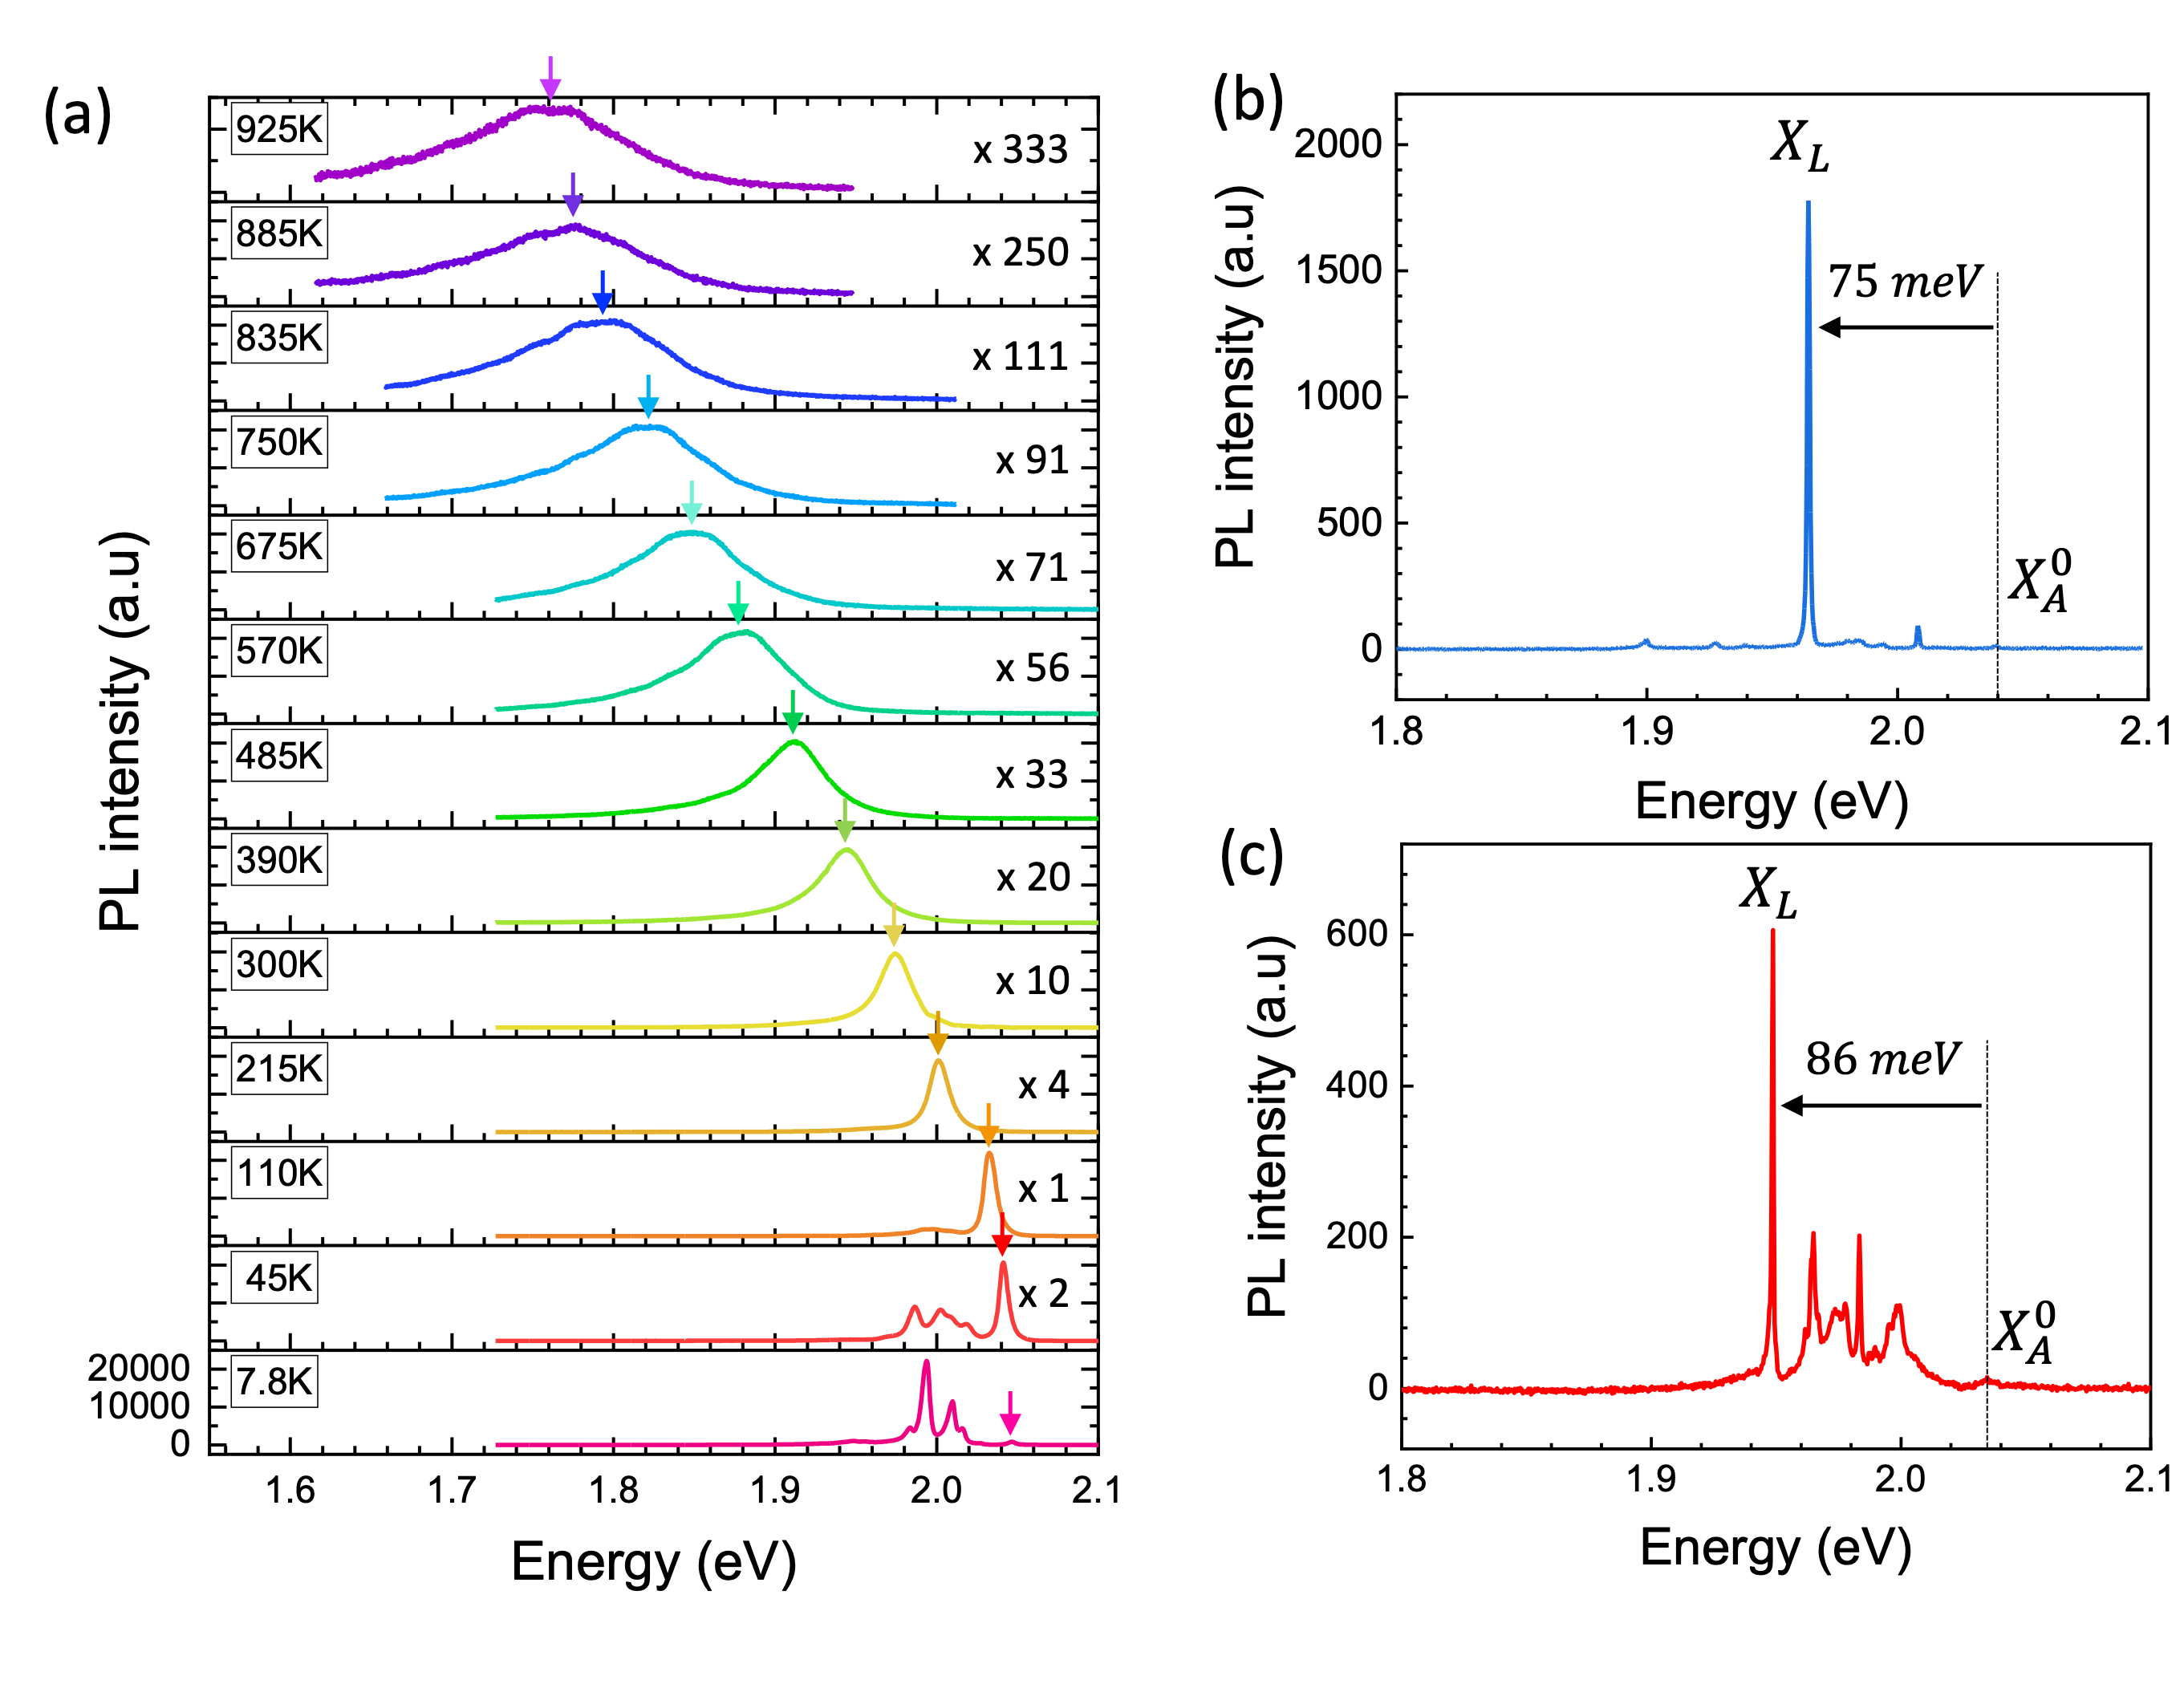
\includegraphics[width=\textwidth]{Figure/Chapter_five/pl_xd_emergence.png}
%     \caption{(a) PL spectra of an hBN-encapsulated WS$_2$ monolayer measured at increasing temperatures from 7.8~K to 925~K ($\lambda_{\mathrm{laser}} = 514$~nm, $P = 1$~$\mu$W), showing a progressive redshift of all excitonic peaks. (b,c) PL spectra after annealing above $\sim$1100~K on two representative chips: (b) chip 3-1, showing $X_D$ at 1.964~eV, and (c) chip 3-4, showing $X_D$ at 1.945~eV. In both cases, the energy offset below $X_A^0$ falls in the range 75--86~meV.}
%     \label{fig:pl_xd_emergence}
% \end{figure}
% Source: Published paper / main paper data.
%   (a) Temperature-dependent PL from 7.8K to 925K (lambda=514nm, P=1uW).
%   (b) Chip 3-1 PL after >1100K annealing, X_D at 1.964 eV.
%   (c) Chip 3-4 PL after >1100K annealing, X_D at 1.945 eV.

\subsection{Sub-meV Linewidth and Spectral Isolation}
\label{subsec:Sub-meV Linewidth and Spectral Isolation}

The most remarkable property of $X_D$ is its spectral narrowness. Fig.~\ref{fig:linewidth_xd} shows PL spectra of the $X_D$ peak (chip 3-4, 1.945~eV) recorded at decreasing excitation powers using the 1800~gr/mm grating of the double spectrometer (instrumental spectral resolution $\approx 0.15$--0.20~meV).

At the highest measured power ($P = 5$~$\mu$W), the $X_D$ peak has a FWHM of approximately 0.6~meV. As the power is systematically reduced, the linewidth narrows monotonically, reaching $\approx 0.2$~meV at the lowest measured power ($P = 0.06$~$\mu$W). This value matches the instrumental resolution limit of the spectrometer, indicating that the true intrinsic linewidth of $X_D$ is at or below 0.2~meV. The power-dependent broadening observed at higher excitation powers is possibly due to local heating induced by the laser.

For comparison, the $X_L$ peak at the same low power has a FWHM of $\sim$2--3~meV---more than an order of magnitude broader than $X_D$ at the same power. This dramatic difference in linewidth indicates that $X_D$ represents a qualitatively different class of emission: a single quantum emitter (or a very small number) with a well-defined, narrow zero-phonon line, rather than an inhomogeneous ensemble.

The spectral isolation of $X_D$ from the intrinsic WS$_2$ emission features (which are concentrated above 1.99~eV) is $\gtrsim$25~meV, sufficient for selective spectral filtering in subsequent photon correlation and time-resolved experiments.

% TODO: add power dependence of narrow emission from chip 3-4
% Figure proposition (fig:linewidth_xd): PL spectra of X_D at chip 3-4 at decreasing powers
%   (5, 1, 0.5, 0.1, 0.06 uW), 1800 gr/mm grating. Show FWHM narrowing from ~0.6 meV to ~0.2 meV.
%   Source: Published paper / main paper data.

\subsection{Power Dependence and Linewidth Broadening}
\label{subsec:Power Dependence and Linewidth Broadening}

Having established the spectral narrowness of $X_D$, we characterize its intensity saturation behavior under two complementary excitation conditions: continuous-wave (CW) excitation on chip 3-1 and pulsed excitation at 78~MHz repetition rate on chip 3-4. Both datasets are shown in Fig.~\ref{fig:power_dep_xd}.

Fig.~\ref{fig:power_dep_xd}(a) shows the CW power dependence of the $X_D$ emission on chip 3-1. The integrated intensity follows the standard two-level CW saturation model,
\begin{equation}
I_{PL}(P) = I_\infty \cdot \frac{P}{P + P_{\mathrm{sat}}^{\mathrm{CW}}},
\label{eq:cw_saturation}
\end{equation}
which arises from the steady-state solution of the rate equations for a two-level emitter under continuous illumination. A fit to Eq.~\ref{eq:cw_saturation} yields $P_{\mathrm{sat}}^{\mathrm{CW}} \approx 5.9~\mu$W, above which the emission saturates. The linewidth of $X_D$ remains near the spectrometer resolution limit ($\sim$0.9~meV) at low powers and broadens monotonically above $\sim$6~$\mu$W, possibly due to local heating induced by the laser.

Fig.~\ref{fig:power_dep_xd}(b) shows the pulsed power dependence of $X_D$ on chip 3-4. The data clearly show sub-linear growth at intermediate powers and saturation at high powers, consistent with the behavior of a quantum two-level emitter under pulsed excitation. In the saturation regime, only one photon per laser pulse can be emitted, as the emitter lifetime ($\sim$900~ps) is much longer than the laser pulse duration (40~ps), and much shorter than the interval between laser pulses (12.8~ns). The PL intensity in the saturation regime is therefore
\begin{equation}
I_{\mathrm{PL}}\ (\mathrm{s}^{-1}) = f_{\mathrm{rep}}\, \Phi_y\, \eta_{\mathrm{opt}}, \qquad \text{(saturation regime)}
\end{equation}
Outside the saturation regime, the probability that the emitter is excited during a laser pulse ($P_{\mathrm{exc}}$) must be considered, so that
\begin{equation}
I_{\mathrm{PL}}\ (\mathrm{s}^{-1}) = P_{\mathrm{exc}}\, f_{\mathrm{rep}}\, \Phi_y\, \eta_{\mathrm{opt}}.
\end{equation}
If $P_\gamma$ denotes the probability that a single photon excites the emitter, the excitation probability can be expressed as
\begin{equation}
P_{\mathrm{exc}} = 1 - (1 - P_\gamma)^{N_\gamma},
\end{equation}
where $N_\gamma$ is the number of laser photons per pulse. For $P_\gamma \ll 1$, this approximates to
\begin{equation}
P_{\mathrm{exc}} \simeq 1 - e^{-N_\gamma P_\gamma},
\end{equation}
and the power-dependent PL intensity of $X_D$ can be fitted using the exponential form
\begin{equation}
I_{X_D}(P_{\mathrm{avg}}) \propto 1 - e^{-\frac{\alpha}{f_{\mathrm{rep}}} P_{\mathrm{avg}}}, \qquad P_\gamma = \alpha h\nu.
\label{eq:saturation}
\end{equation}
From the exponential fit to the data in Fig.~\ref{fig:power_dep_xd}(b), $\alpha = 6.92 \times 10^{12}$~J$^{-1}$, yielding $P_\gamma = \alpha h\nu = 2.73 \times 10^{-6}$ and a pulsed saturation power $f_{\mathrm{rep}}/\alpha \approx 11.3~\mu$W. The quantum yield $\Phi_y$ is extracted directly in the saturation regime as
\begin{equation}
\mathrm{QY} = \frac{R_{\mathrm{APD1}} + R_{\mathrm{APD2}}}{f_{\mathrm{rep}}\, \eta_{\mathrm{opt}}},
\end{equation}
where $R_{\mathrm{APD1}}$ and $R_{\mathrm{APD2}}$ are the photon count rates detected by the two SPADs. Using a total detected count rate of 1000~counts/s and $\eta_{\mathrm{opt}} = 2.44 \times 10^{-4}$, the quantum yield is estimated to be $\sim$5.25\%. The linewidth of $X_D$ remains near the resolution-limited value of $\lesssim 0.2$~meV at low excitation powers and begins to broaden above $\sim$1~$\mu$W (Fig.~\ref{fig:power_dep_xd}(b), right axis), possibly due to local heating induced by the laser.

% \begin{figure}[htbp]
%     \centering
%     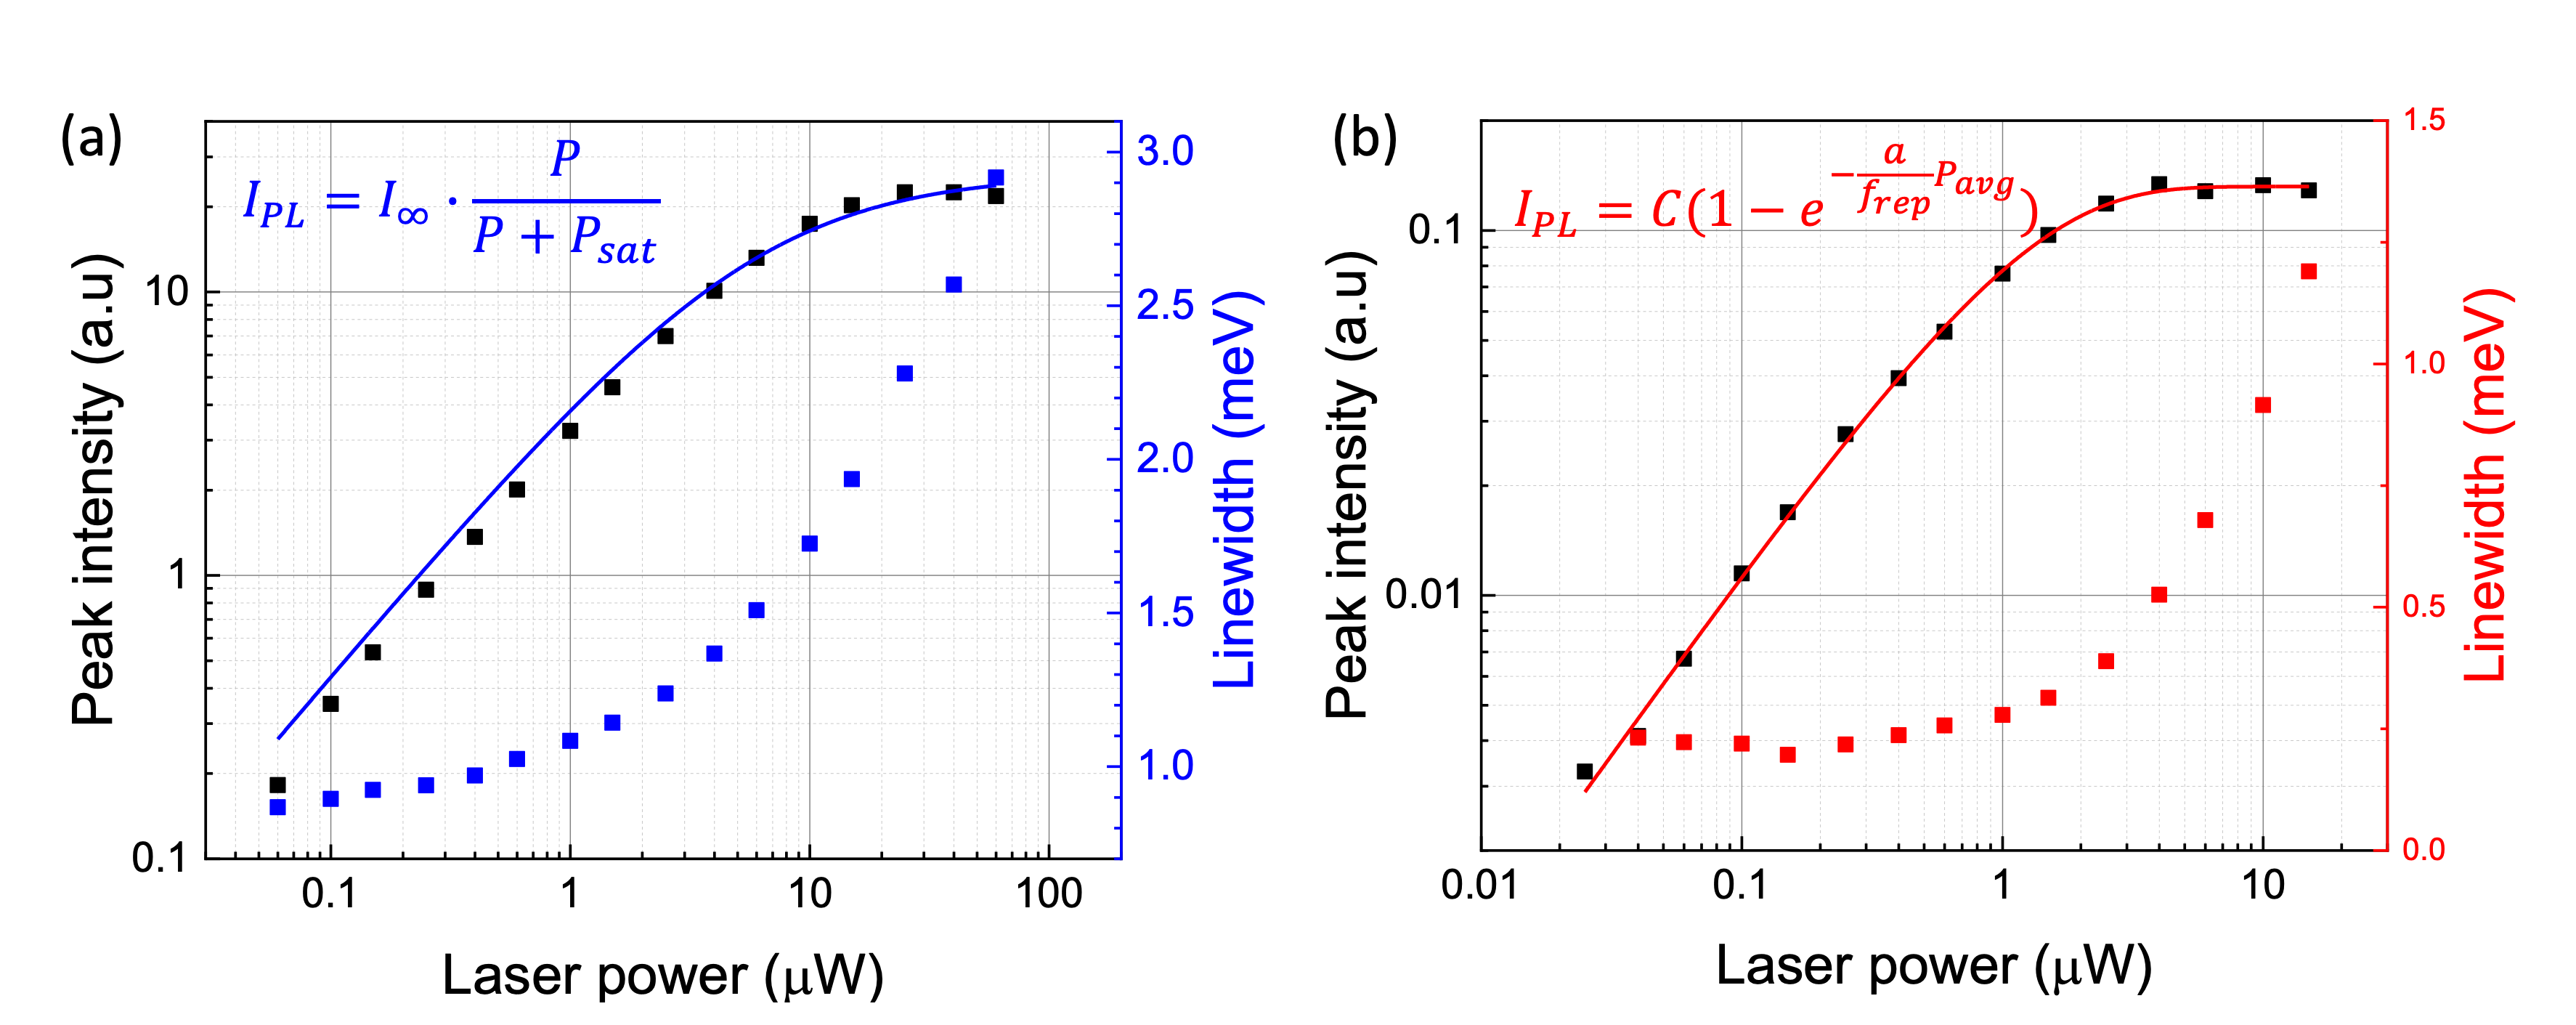
\includegraphics[width=\textwidth]{Figure/Chapter_five/power_dep_xd.png}
%     \caption{Power dependence of the $X_D$ peak integrated intensity (left axis) and linewidth (right axis). (a) CW excitation (chip 3-1, $T = 3.64$~K). The solid line is a fit to the CW saturation model (Eq.~\ref{eq:cw_saturation}), yielding $P_{\mathrm{sat}}^{\mathrm{CW}} \approx 5.9~\mu$W. (b) Pulsed excitation (78~MHz, chip 3-4, $T = 3.64$~K). The solid line is a fit to the exponential saturation model (Eq.~\ref{eq:saturation}), yielding $\alpha = 6.92 \times 10^{12}$~J$^{-1}$ ($P_{\mathrm{sat}}^{{\mathrm{pulsed}}} = f_{\mathrm{rep}}/\alpha \approx 11.3~\mu$W, QY $\approx 5.25\%$). In both cases the linewidth broadens at elevated powers, possibly due to local laser heating.}
%     \label{fig:power_dep_xd}
% \end{figure}
% Source: Published paper / main paper data.
%   (a) CW power dependence, chip 3-1, T=3.64K. Saturation model fit: P_sat^CW ~ 5.9 uW.
%   (b) Pulsed 78 MHz power dependence, chip 3-4, T=3.64K. Exponential fit: alpha=6.92e12 J^-1,
%       P_sat^pulsed ~ 11.3 uW, QY ~ 5.25%. Right axis: linewidth vs power.

\subsection{PLE Spectroscopy: WS$_2$ Origin}
\label{subsec:PLE Spectroscopy WS2 Origin}

The sub-meV linewidth of $X_D$ and its 75--86~meV offset below the neutral exciton raise the question of whether this feature is intrinsic to WS$_2$ or could arise from defects in the surrounding hBN or SiC layers. To resolve this, we performed PLE spectroscopy with the detection window centered on the $X_D$ peak.

Fig.~\ref{fig:ple_xd} shows the PLE spectra recorded on chip 3-1 at $T = 3.66$~K and $P = 10$~$\mu$W, with detection at the $X_D$ energy (1.964~eV), and on chip 3-4 at $T = 3.64$~K and $P = 1$~$\mu$W, with detection at the $X_D$ energy (1.945~eV). The excitation wavelength was scanned from 400~nm to 600~nm and 450~nm to 620~nm for each sample.

The PLE spectrum displays a clear set of resonances that are immediately recognizable as the intrinsic optical transitions of WS$_2$. For chip 3-4, we identify the A-exciton ground state ($X_A^0$: 1s, $\approx 2.033$~eV) with a small Stokes shift compared to the A-exciton peak in the PL spectrum, the A-exciton 2s excited state ($X_A^0$: 2s, $\approx 2.07$~eV), the trion resonance ($T$, $\approx 2.020$~eV), and the B exciton ($X_B^0$, $\approx 2.45$~eV). For chip 3-1, only the B-exciton resonance is visible, as the scanning range is not sufficient to reach the A-exciton resonance. This pattern is identical to the PLE spectrum of the pristine sample (Section~\ref{subsec:PLE Spectroscopy Exciton and Excited States}) and of the $X_L$ emission (Section~\ref{subsec:PLE Spectroscopy Intrinsic WS2 Resonances}), confirming that $X_D$ shares the same absorption channels as the intrinsic excitonic emission. No features attributable to hBN or SiC are present.

The consistent identification of WS$_2$ excitonic resonances in the PLE of $X_D$, combined with the absence of any hBN or SiC fingerprints, provides clear spectroscopic evidence that $X_D$ is an intrinsic emission channel of the WS$_2$ monolayer, arising from excitons that are absorbed in the WS$_2$ band, relax, diffuse, and become trapped at a specific class of thermally activated defect sites.

% \begin{figure}[htbp]
%     \centering
%     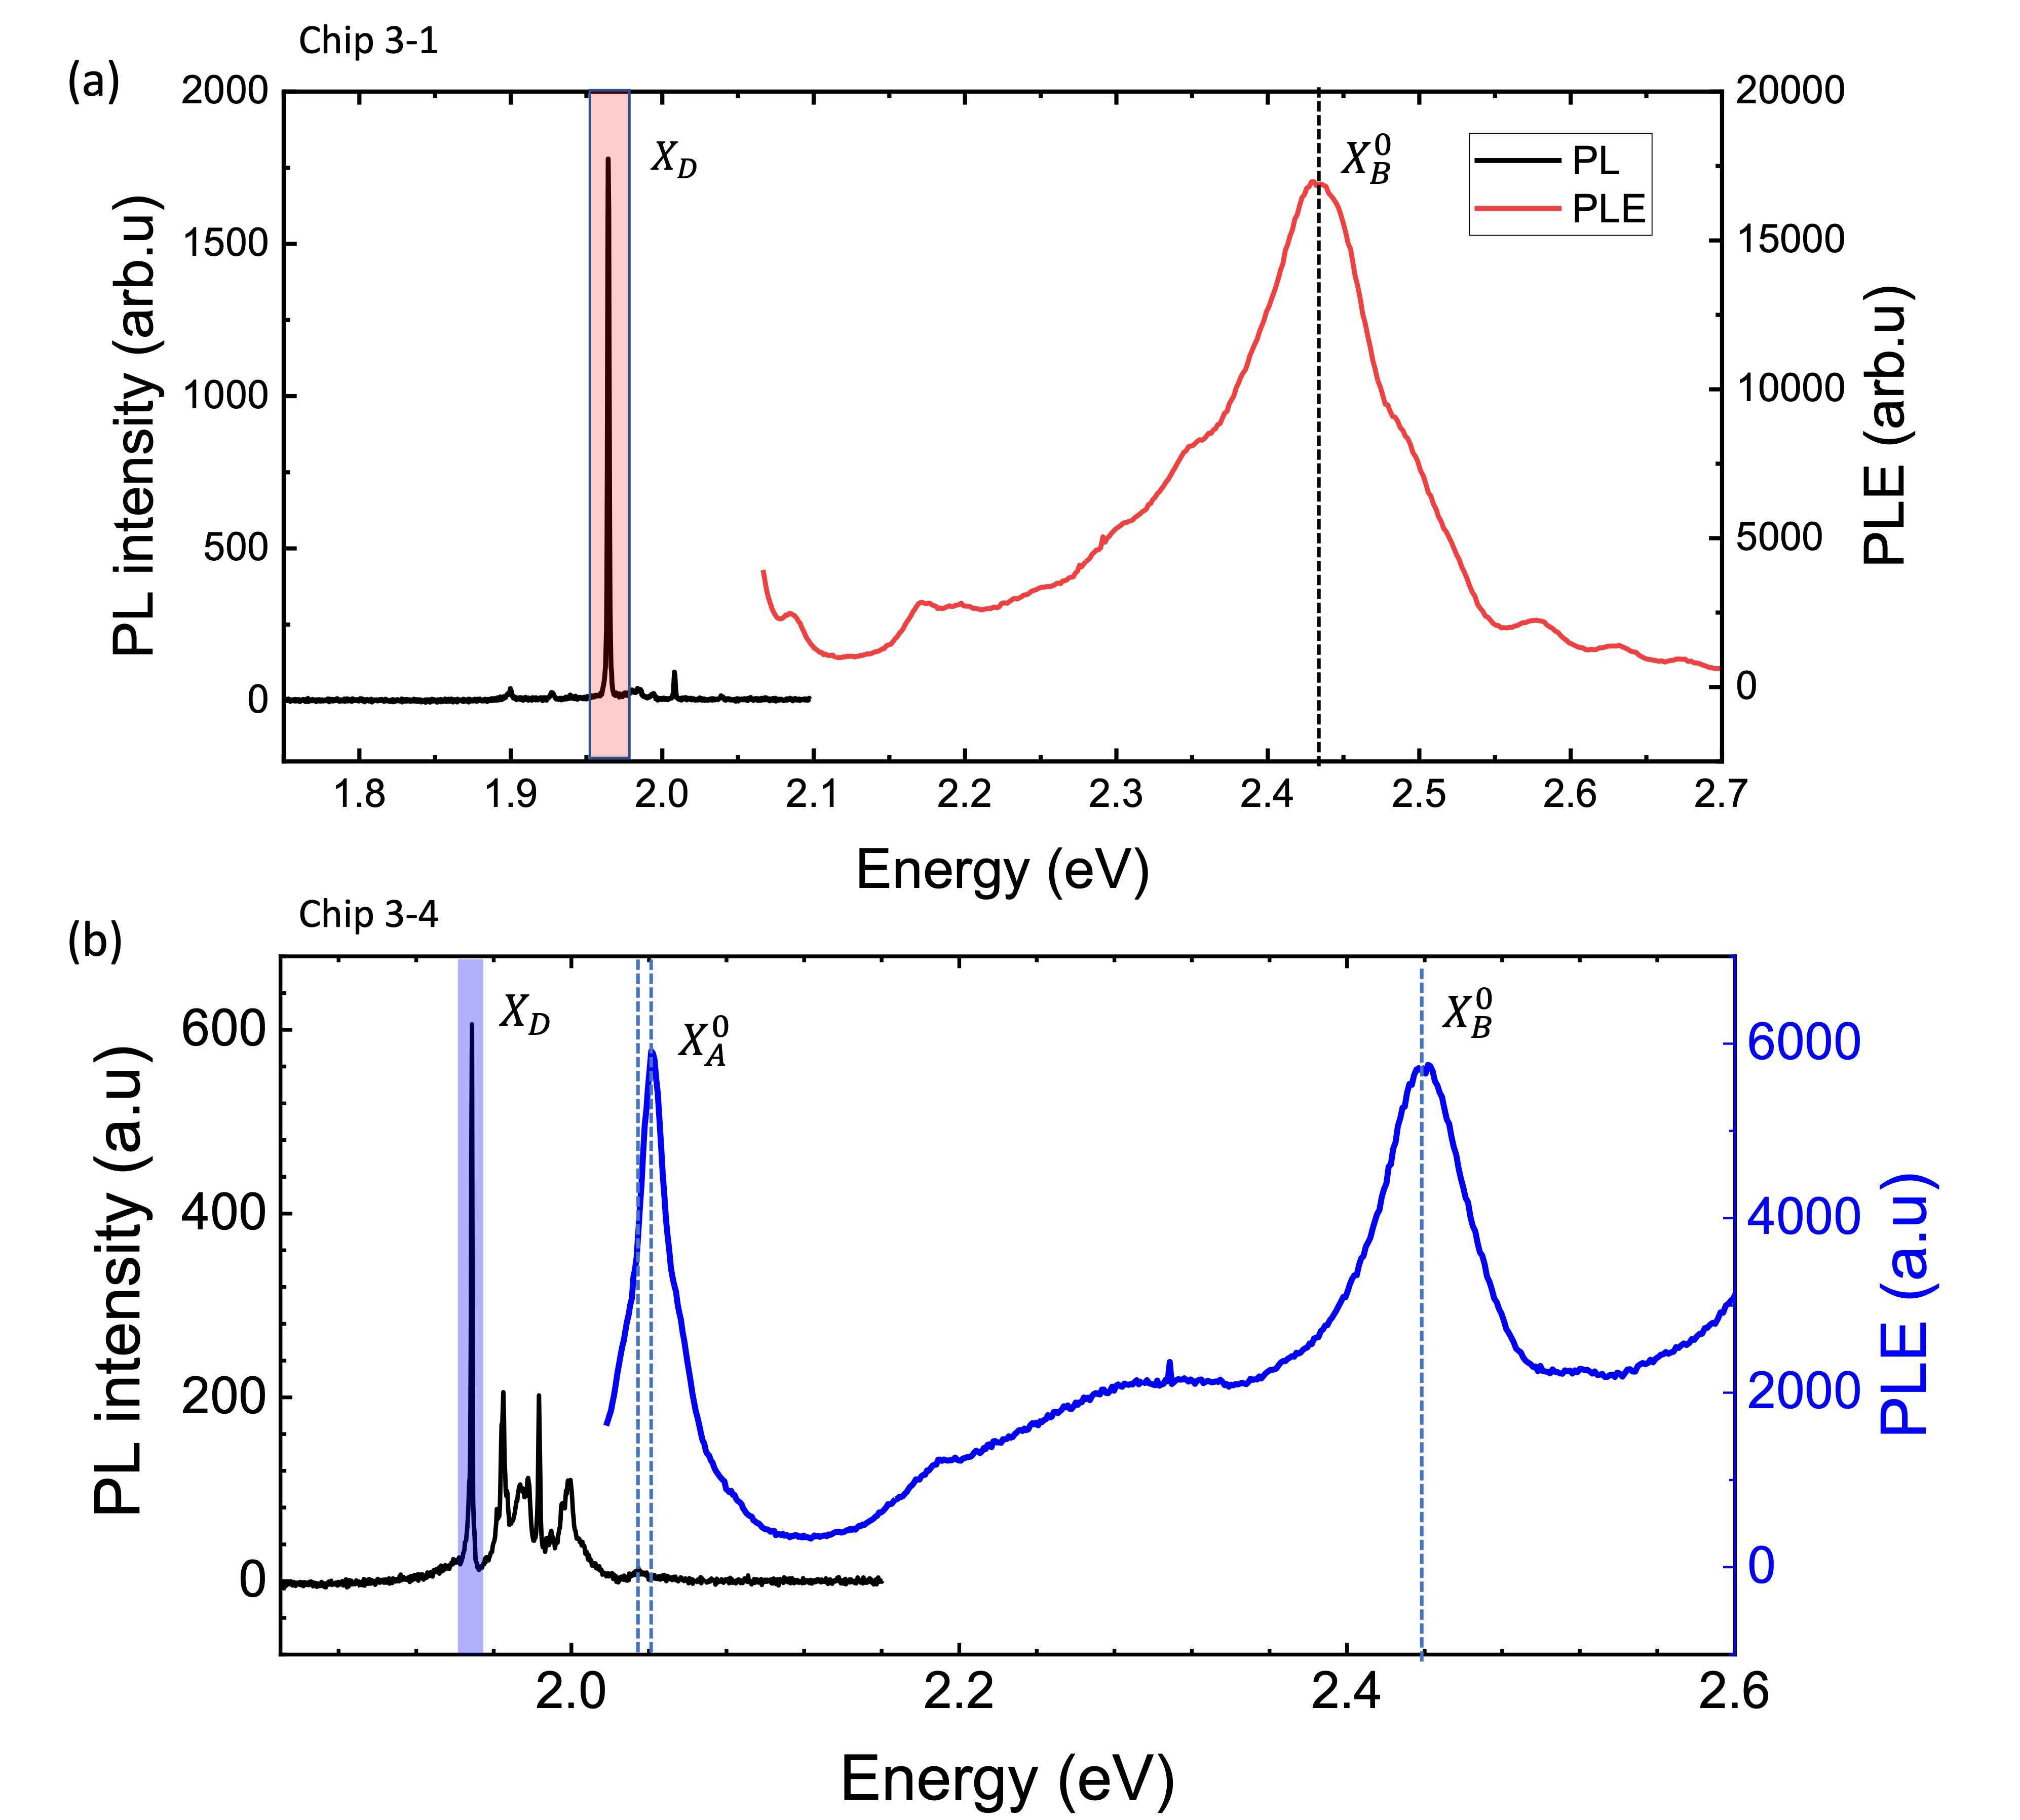
\includegraphics[width=\textwidth]{Figure/Chapter_five/ple_xd.png}
%     \caption{PLE spectra of the $X_D$ emission. (a) Chip 3-1 (detection at 1.964~eV, $T = 3.66$~K, $P = 10$~$\mu$W), showing the B-exciton resonance ($X_B^0$). (b) Chip 3-4 (detection at 1.945~eV, $T = 3.64$~K, $P = 1$~$\mu$W), showing resonances at $X_A^0$ (1s), $X_A^0$ (2s), trion ($T$), and $X_B^0$, confirming the intrinsic WS$_2$ origin of $X_D$.}
%     \label{fig:ple_xd}
% \end{figure}
% Source: Published paper / main paper data.
%   (a) Chip 3-1, detection at X_D = 1.964 eV, T=3.66K, P=10uW, scan 400-600 nm. Shows X_B^0.
%   (b) Chip 3-4, detection at X_D = 1.945 eV, T=3.64K, P=1uW, scan 450-620 nm.
%       Resonances: X_A^0 1s (~2.033 eV), X_A^0 2s (~2.07 eV), trion (~2.020 eV), X_B^0 (~2.45 eV).

\subsection{Time-Resolved PL: Single-Exponential Decay and Nanosecond Lifetime}
\label{subsec:Time-Resolved PL Nanosecond Lifetime}

The PLE measurements confirm that $X_D$ emission originates from the WS$_2$ layer. To further characterize the emitter, we performed time-resolved photoluminescence (TRPL) measurements on chip 3-1 and chip 3-4 to determine the radiative lifetime of $X_D$. The laser pulse duration is 40~ps and the repetition period is 12.8~ns (78~MHz).

Fig.~\ref{fig:trpl_xd_3_1}(a) shows the TRPL time-energy map recorded on chip 3-1 at $T = 3.64$~K with $\lambda_{\mathrm{laser}} = 514$~nm and $P = 1$~$\mu$W. The temporal profiles of $X_D$ and the trion are compared directly on a linear scale in Fig.~\ref{fig:trpl_xd_3_1}(b). The trion decays with $\tau_{\mathrm{trion}} \approx 600$~ps, whereas $X_D$ exhibits distinctly different dynamics: its onset is delayed by approximately 130~ps relative to the trion peak, followed by a slow decay extending over several nanoseconds. The semi-logarithmic decay trace in Fig.~\ref{fig:trpl_xd_3_1}(c) confirms that the $X_D$ decay is well described by a single exponential $I(t) \propto \exp(-t/\tau)$ with $\tau \approx 2$~ns.

% \begin{figure}[htbp]
%     \centering
%     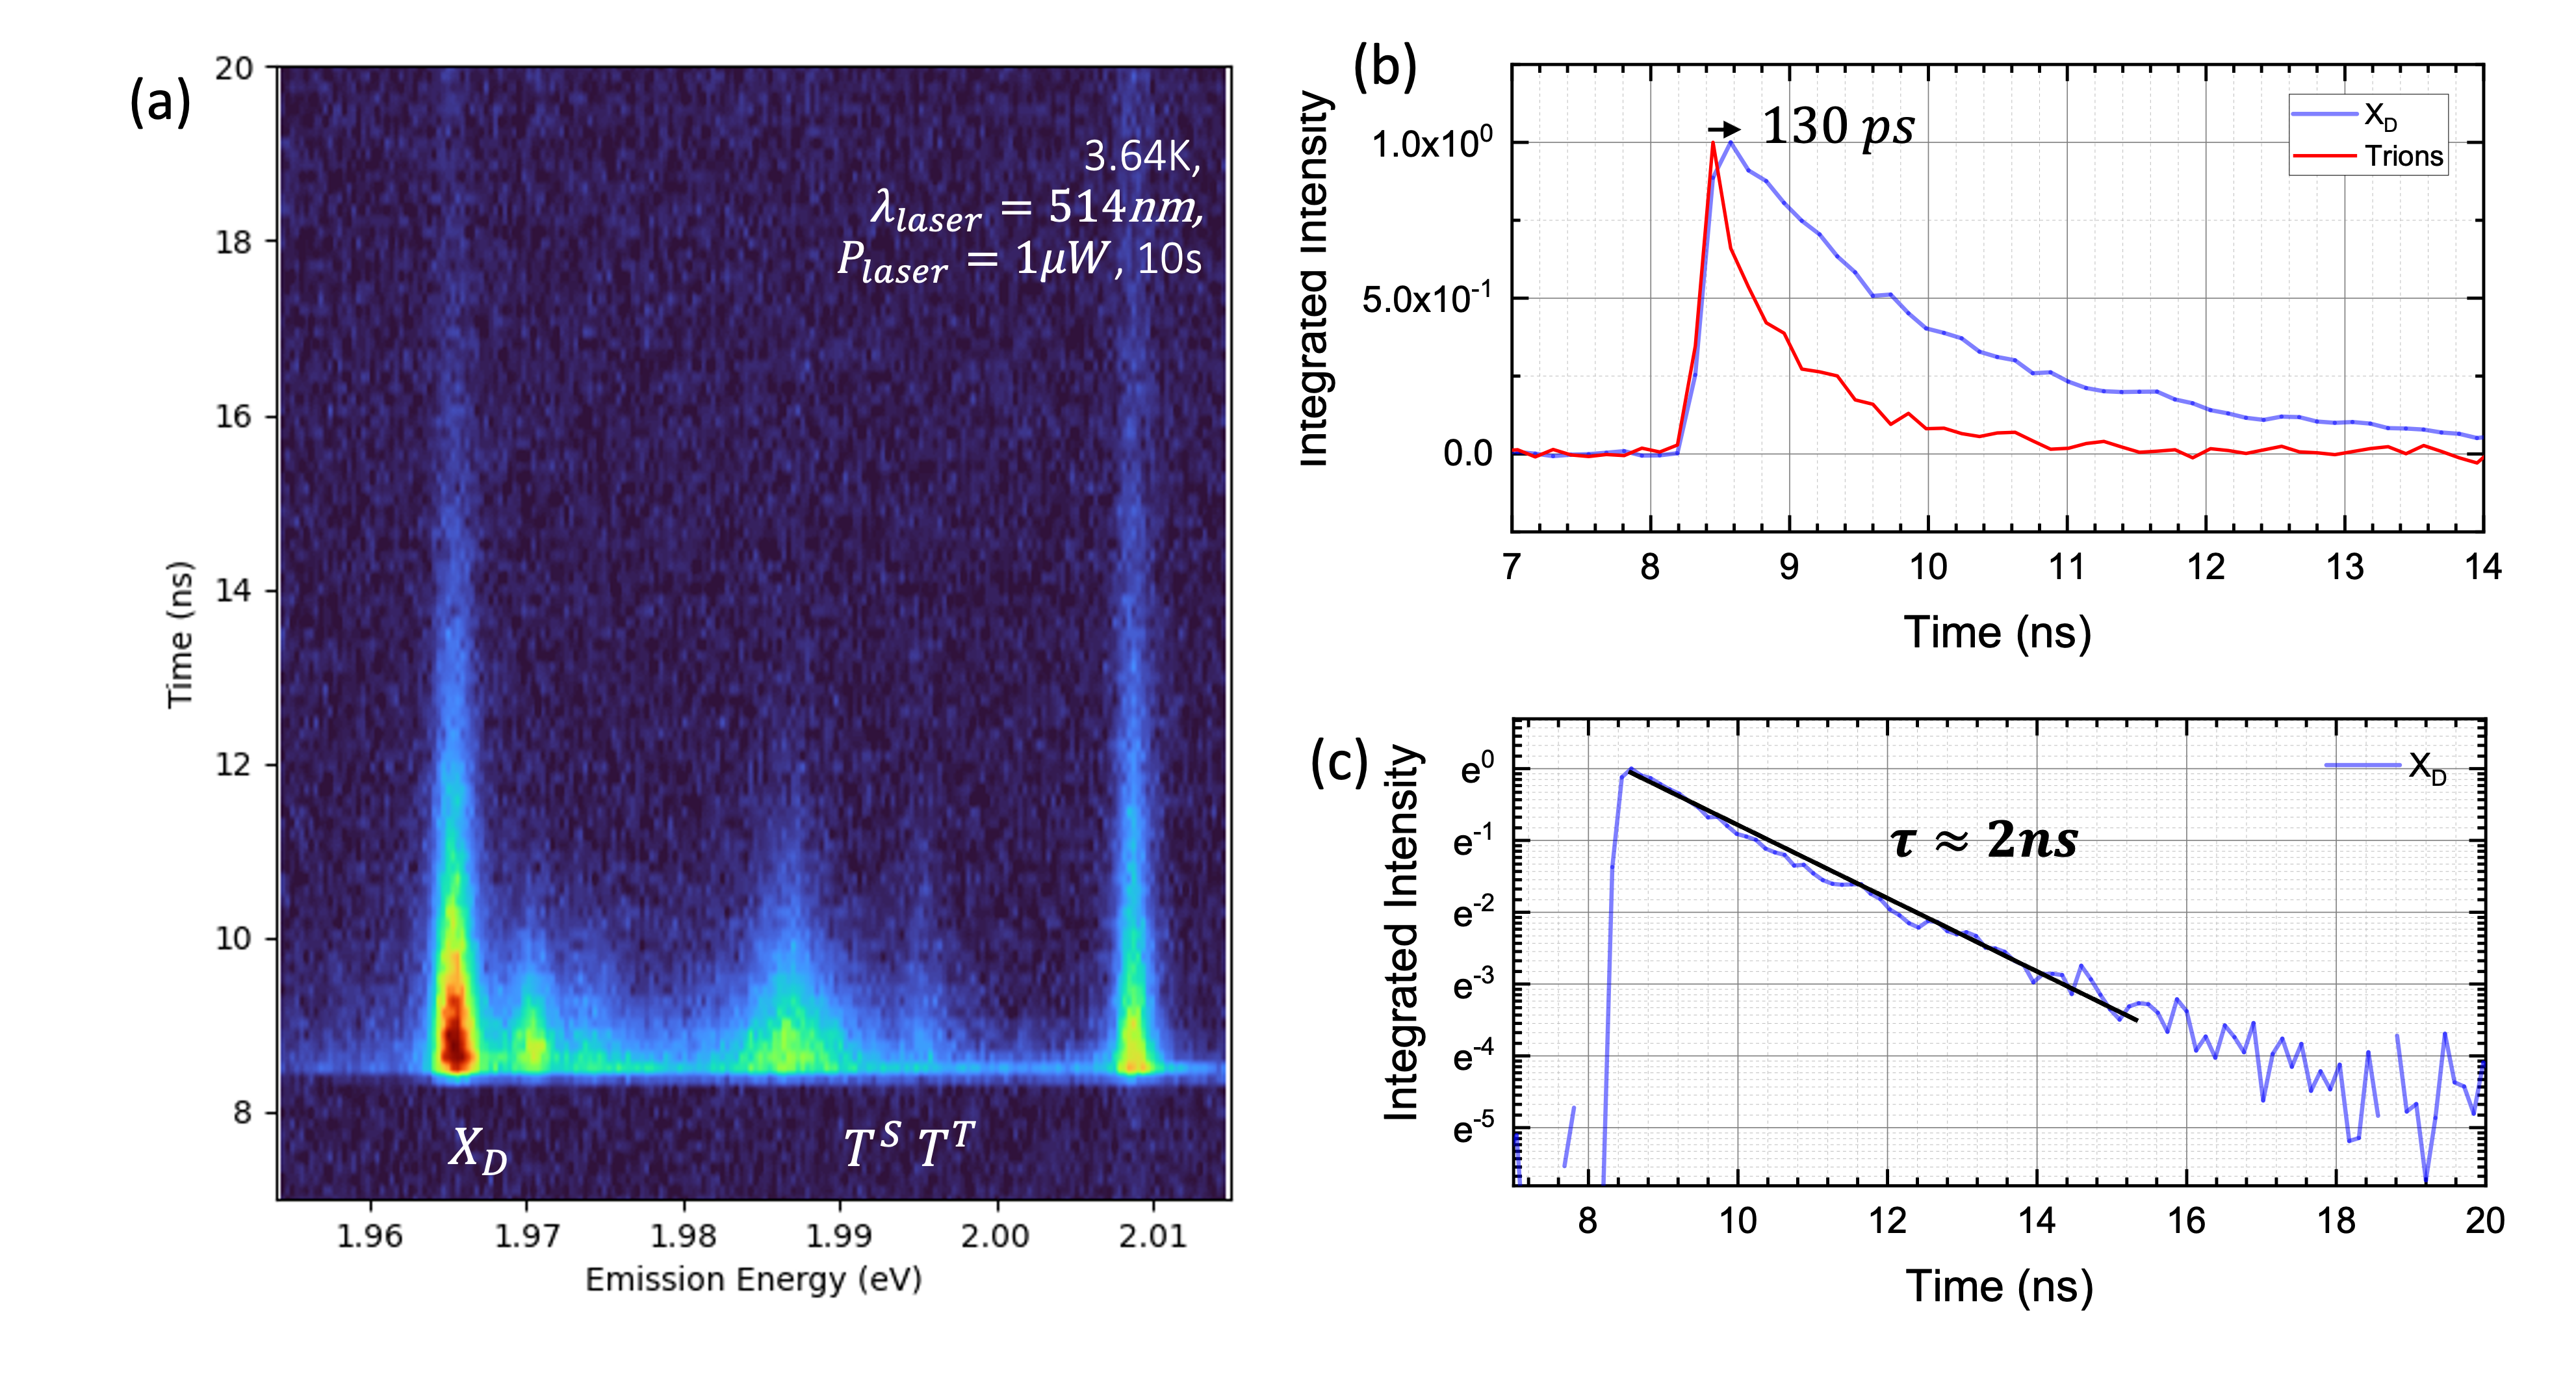
\includegraphics[width=\textwidth]{Figure/Chapter_five/trpl_xd_3_1.png}
%     \caption{TRPL of $X_D$ on chip 3-1 ($T = 3.64$~K, $\lambda_{\mathrm{laser}} = 514$~nm, $P = 1$~$\mu$W). (a) Time--energy map. (b) Linear-scale decay traces of $X_D$ and the trion, highlighting the $\sim$130~ps delayed onset of $X_D$ relative to the trion peak. (c) Semi-logarithmic decay trace of $X_D$ with a single-exponential fit, yielding $\tau \approx 2$~ns.}
%     \label{fig:trpl_xd_3_1}
% \end{figure}
% Source: Published paper / main paper data.
%   Chip 3-1, T=3.64K, lambda=514nm, P=1uW.
%   (a) Time-energy map (time axis ~0-10 ns, energy axis ~1.93-2.06 eV).
%   (b) Linear decay traces: trion tau~600ps, X_D onset delayed ~130ps vs trion peak.
%   (c) Semi-log decay of X_D with single-exponential fit, tau~2 ns.

TRPL measurements were also performed on chip 3-4, which serves as the primary sample for this chapter. Fig.~\ref{fig:trpl_xd_3_4}(a) shows the corresponding time-energy map, with the energy axis covering 1.92--2.06~eV. The intrinsic excitonic emission (trion, dark trion at 1.99--2.05~eV) decays within $\sim$200~ps, while the $X_D$ emission at $\sim$1.945~eV exhibits distinctly different dynamics: its onset is delayed by approximately 200~ps relative to the laser pulse, followed by a gradual rise and a slow decay extending across several nanoseconds. The semi-logarithmic decay trace in Fig.~\ref{fig:trpl_xd_3_4}(c) yields a single-exponential lifetime of $\tau \approx 0.9$~ns.

% \begin{figure}[htbp]
%     \centering
%     \includegraphics[width=\textwidth]{Figure/Chapter_five/trpl_xd_3_4.png}
%     \caption{TRPL of $X_D$ on chip 3-4 ($T = 3.64$~K, $\lambda_{\mathrm{laser}} = 503$~nm, $P = 1$~$\mu$W). (a) Time--energy map showing the fast decay of trion/exciton emission and the delayed onset and slow decay of $X_D$. (b) Time-averaged PL spectrum indicating the spectral window of $X_D$. (c) Semi-logarithmic decay trace of $X_D$ with a single-exponential fit, yielding $\tau \approx 0.9$~ns.}
%     \label{fig:trpl_xd_3_4}
% \end{figure}
% Source: Published paper / main paper data.
%   Chip 3-4, T=3.64K, lambda=503nm, P=1uW.
%   (a) Time-energy map, energy 1.92-2.06 eV. Trion/dark trion decay <200ps; X_D onset ~200ps.
%   (b) Time-averaged PL spectrum showing X_D at ~1.945 eV.
%   (c) Semi-log decay of X_D with single-exponential fit, tau~0.9 ns.

The delayed onset of $X_D$---observed on both chips---reflects the two-step nature of the excitation: photons are first absorbed by the WS$_2$ lattice, generating free excitons which then diffuse through the monolayer until captured by the $X_D$ defect site. This is consistent with the $\sim$200~ps delay observed for $X_L$ in chip 2-10 (Chapter~\ref{chap:four}), suggesting that the exciton diffusion and capture dynamics are a common feature of thermally activated defect emission in WS$_2$. The nanosecond-scale lifetimes of $X_D$---$\tau \approx 2$~ns on chip 3-1 and $\tau \approx 0.9$~ns on chip 3-4---are significantly longer than the $X_L$ emission ($\tau \approx 513$~ps in chip 2-10, Chapter~\ref{chap:four}), consistent with the nanosecond lifetimes typically reported for single-photon emitters in 2D materials. As the emitter lifetime is much longer than the laser pulse duration (40~ps) and much shorter than the repetition period (12.8~ns), $X_D$ is well placed in the ideal regime for single-photon operation, motivating the photon correlation measurements presented in the following section.


\section{Quantum Optical Characterization: Second-Order Photon Correlations}
\label{sec:Quantum Optical Characterization: Second-Order Photon Correlations}

The preceding sections have established that $X_D$ is a spectrally isolated, ultra-narrow, long-lifetime emission channel of WS$_2$ origin. These properties are all necessary conditions for single-photon emission, but not sufficient: a true single-photon source can emit at most one photon per excitation event, which is a fundamentally non-classical property. The definitive experimental test is the measurement of the second-order photon correlation function $g^{(2)}(\tau)$, which directly quantifies the probability of detecting two photons simultaneously.

\subsection{Hanbury Brown--Twiss Interferometry}
\label{subsec:Hanbury Brown-Twiss Interferometry}

The second-order photon correlation function is defined as

\begin{equation}
g^{(2)}(\tau) = \frac{\langle I(t)\, I(t+\tau) \rangle}{\langle I(t)\rangle^2},
\label{eq:g2}
\end{equation}

where $I(t)$ denotes the instantaneous photon detection rate and $\langle \cdot \rangle$ denotes a time average. For a perfectly coherent (laser) light source, $g^{(2)}(\tau) = 1$ for all $\tau$. For a thermal (chaotic) source, $g^{(2)}(0) = 2$ (photon bunching). For a perfect single-photon emitter, $g^{(2)}(0) = 0$ (photon antibunching), reflecting the impossibility of emitting two photons simultaneously. The conventional threshold for claiming single-photon emission is $g^{(2)}(0) < 0.5$, which cannot be reached by any mixture of coherent sources.

Fig.~\ref{fig:hbt_setup} illustrates the Hanbury Brown--Twiss (HBT) interferometer used in this work. The emission from $X_D$, spectrally filtered by the double spectrometer to isolate the $X_D$ peak, is directed into a 50:50 non-polarizing beamsplitter that divides the photon stream into two paths. Each path terminates at a single-photon avalanche photodiode (SPAD, temporal jitter $\approx 30$~ps). The arrival times of detection events on both SPADs are recorded by a time-correlated single-photon counting (TCSPC) module, which accumulates a histogram of the time difference $\tau$ between start events (SPAD 1) and stop events (SPAD 2). This histogram, after normalization to the uncorrelated background level, yields $g^{(2)}(\tau)$.

Under pulsed excitation at 78~MHz, the $g^{(2)}(\tau)$ histogram takes the form of a comb of peaks separated by the laser repetition period $T_{\mathrm{rep}} = 1/f_{\mathrm{rep}} = 12.8$~ns. Each peak corresponds to coincidences from photons in the same or successive excitation cycles. For an ideal single-photon emitter, the central peak at $\tau = 0$ (same excitation cycle) vanishes, since two photons cannot be emitted in the same cycle. For a realistic emitter with background emission, the central peak is suppressed relative to the side peaks by a factor that depends on the signal-to-background ratio.

% \begin{figure}[htbp]
%     \centering
%     \includegraphics[width=0.8\textwidth]{Figure/Chapter_five/hbt_setup.png}
%     \caption{Schematic of the Hanbury Brown--Twiss (HBT) interferometer. The emission from $X_D$ is spectrally filtered by the double spectrometer and directed onto a 50:50 beamsplitter. Photons are detected by two SPADs, and the arrival-time difference $\tau$ is histogrammed by TCSPC electronics to yield $g^{(2)}(\tau)$.}
%     \label{fig:hbt_setup}
% \end{figure}
% Source: Can reuse the schematic from CSI 2nd year report, Fig. 15(a,b).
%   Diagram: sample -> objective -> spectrometer filter -> 50:50 BS -> SPAD1 + SPAD2 -> TCSPC -> g2(tau) histogram.
%   Include formula g2(tau) = <I(t)I(t+tau)> / <I(t)>^2.

\subsection{Photon Antibunching and $g^{(2)}(0) < 0.5$}
\label{subsec:Photon Antibunching and g2(0) < 0.5}

Fig.~\ref{fig:g2_tau} shows the measured $g^{(2)}(\tau)$ histogram for $X_D$ on chip 3-4, accumulated over 24~hours of continuous pulsed excitation at $\lambda_{\mathrm{laser}} = 506$~nm and $P = 1$~$\mu$W, at $T = 3.64$~K. The extended integration time was necessary to accumulate sufficient coincidence counts given the low detected photon rate at the operating power ($\sim$1000 counts/s per SPAD).

The histogram displays the expected comb of peaks separated by 12.8~ns. Critically, the central peak at $\tau = 0$ is clearly suppressed relative to the side peaks: its integrated area is less than 50\% of the average area of the neighboring peaks. The value of $g^{(2)}(0)$, computed as the ratio of the zero-delay peak area to the mean area of the side peaks, is approximately $g^{(2)}(0) \approx 0.3$--0.4, well below the classical threshold of 0.5. This pronounced antibunching constitutes unambiguous evidence that $X_D$ emits predominantly single photons: it is impossible for a classical or thermal light source to produce $g^{(2)}(0) < 1$, and $g^{(2)}(0) < 0.5$ specifically rules out the possibility that the emission is a mixture of two or more classical sources.

The residual finite value of $g^{(2)}(0) \approx 0.3$--0.4 (rather than the ideal 0) arises from two main contributions. First, background emission from intrinsic excitonic features that fall within the spectrometer collection window introduces uncorrelated photon pairs that increase the measured $g^{(2)}(0)$. In the presence of a background contributing a fraction $\rho$ of the total detected signal, the measured value is related to the true single-emitter value by $g^{(2)}_{\mathrm{meas}}(0) = g^{(2)}_{\mathrm{true}}(0) + 2\rho(1-\rho)$ in the limit of a pure background ($g^{(2)}_{\mathrm{bg}}(0) = 1$), so even a 20--30\% background contribution can raise $g^{(2)}(0)$ from 0 to 0.3--0.4. Second, if multiple $X_D$ emitters reside within the diffraction-limited excitation spot simultaneously, their combined emission would yield $g^{(2)}(0) = 1 - 1/N$ for $N$ indistinguishable emitters, corresponding to $g^{(2)}(0) = 0.5$ for $N = 2$ and smaller values for fewer emitters. The observed $g^{(2)}(0) \approx 0.3$--0.4 is consistent with either a single emitter with moderate background or two emitters with minimal background. Future measurements with near-resonant excitation (to suppress background) and narrower spectral filters are expected to bring $g^{(2)}(0)$ closer to zero.

% \begin{figure}[htbp]
%     \centering
%     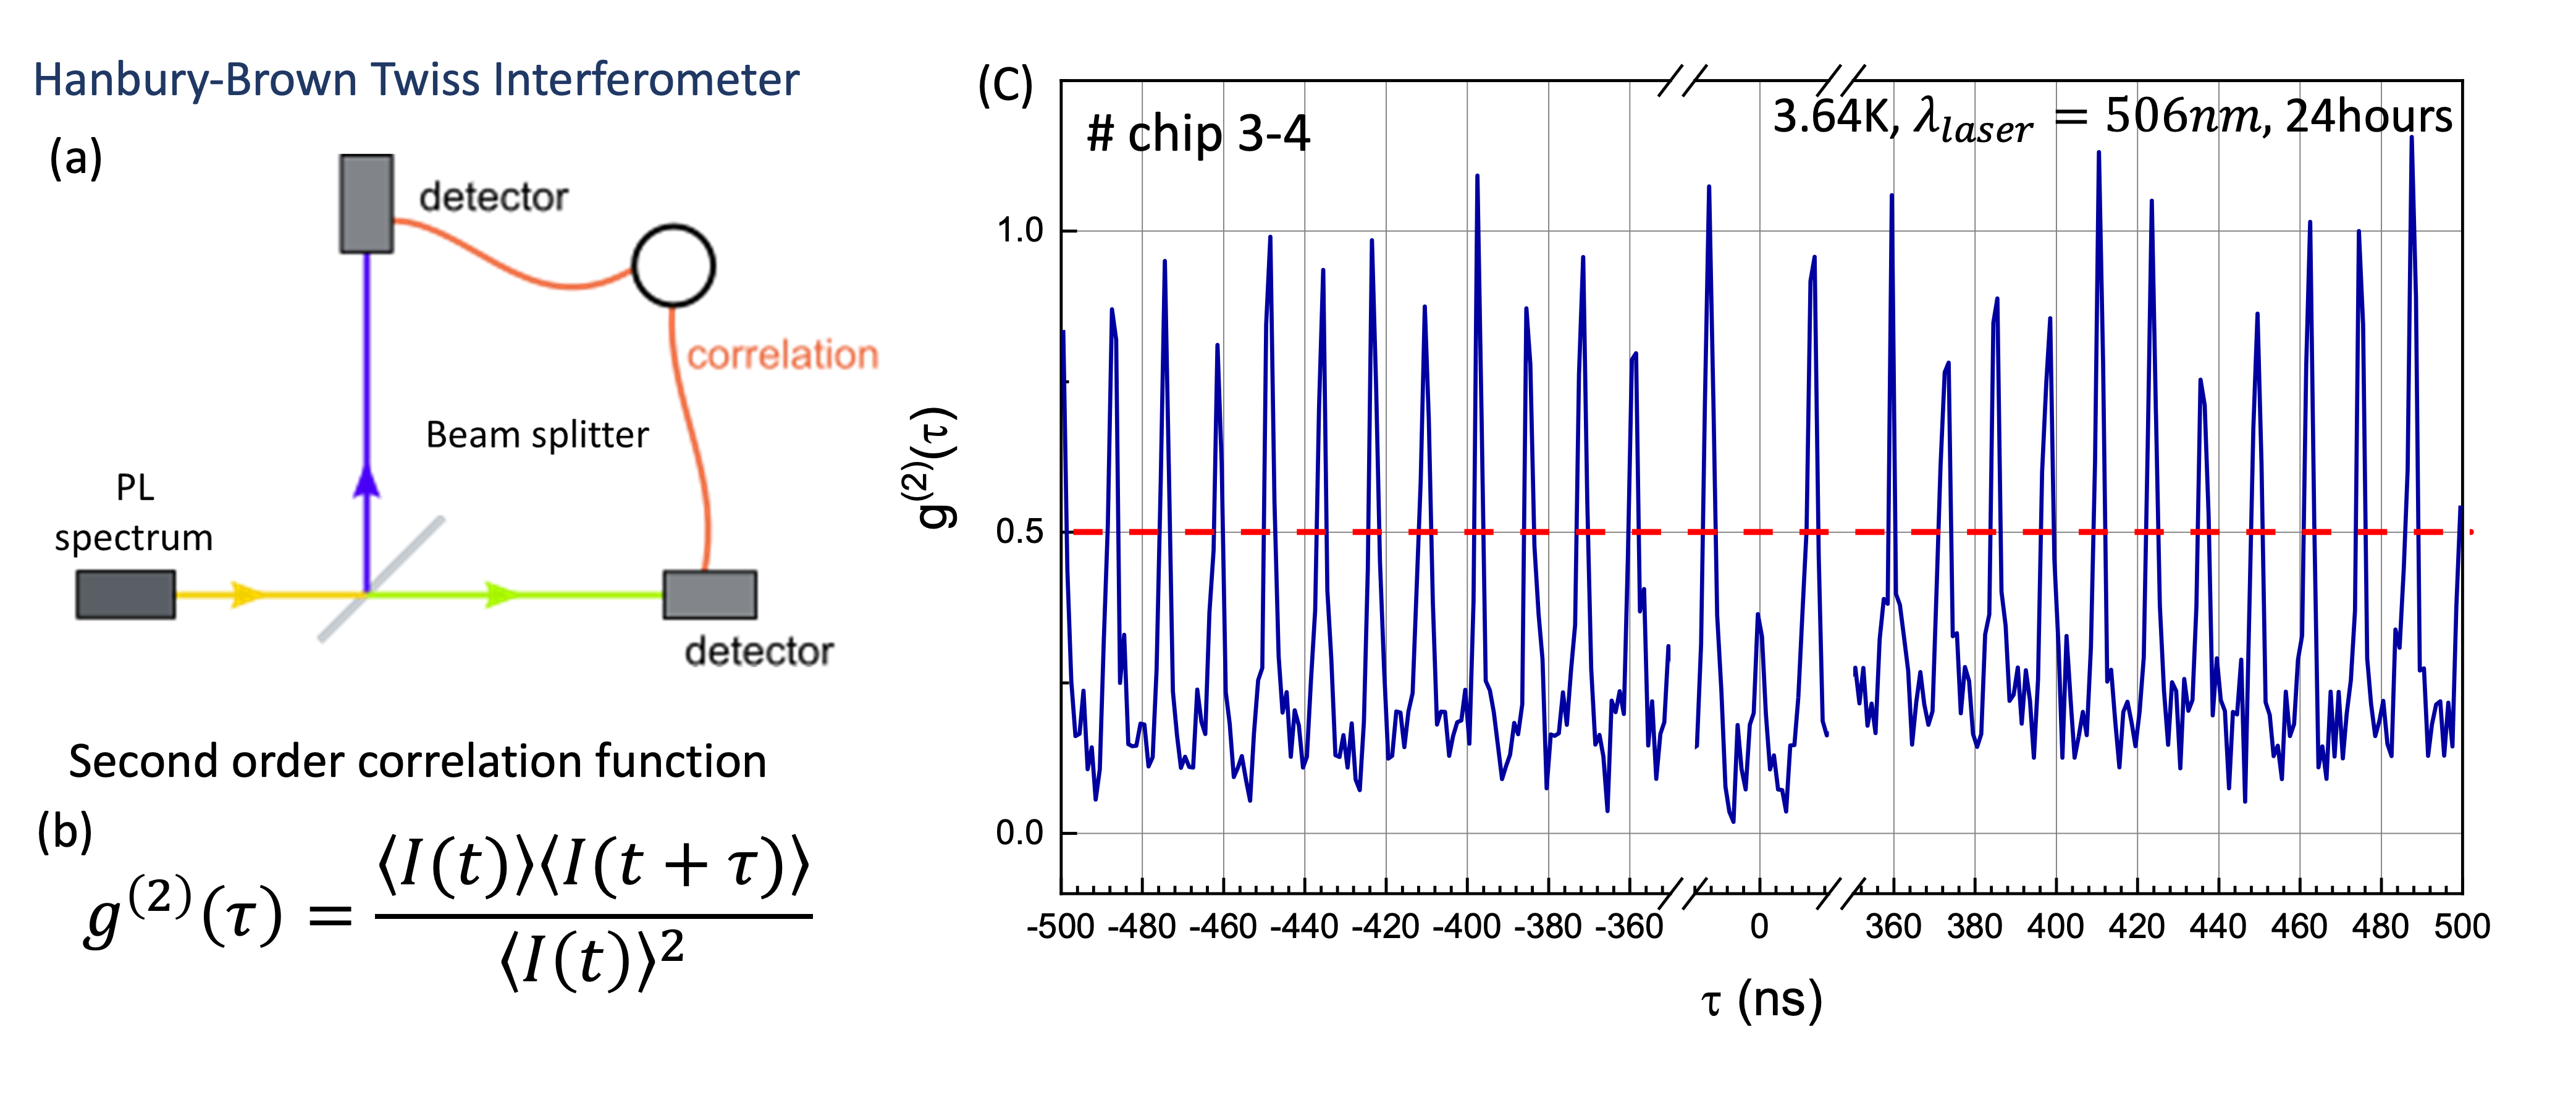
\includegraphics[width=\textwidth]{Figure/Chapter_five/g2_tau.png}
%     \caption{$g^{(2)}(\tau)$ histogram for the $X_D$ emission (chip 3-4) measured under pulsed excitation at 78~MHz, $\lambda_{\mathrm{laser}} = 506$~nm, $P = 1$~$\mu$W, $T = 3.64$~K (24~h integration). The comb of peaks is separated by the laser repetition period (12.8~ns). The central peak at $\tau = 0$ is suppressed to $g^{(2)}(0) \approx 0.3$--0.4, well below the 0.5 threshold (red dashed line), demonstrating single-photon emission from $X_D$.}
%     \label{fig:g2_tau}
% \end{figure}
% Source: Published paper / main paper data; CSI 2nd year report Fig. 15(c).
%   Chip 3-4, pulsed 78 MHz, lambda=506nm, P=1uW, T=3.64K, 24h integration.
%   tau axis: -500 to +500 ns. Peaks at 12.8 ns spacing. Central peak g2(0)~0.3-0.4.
%   Add red dashed horizontal line at g2=0.5.


\subsection{Quantum Yield and Detection Efficiency}
\label{subsec:Quantum Yield and Detection Efficiency}

In addition to the photon purity established by $g^{(2)}(0)$, the quantum efficiency of the $X_D$ emitter is a key figure of merit for quantum photonic applications. We estimate the quantum yield (QY) of $X_D$ using the detected photon count rate at the saturation power together with the known optical collection efficiency of the system.

The total detected count rate at saturation is $\sim$1000 counts/s per SPAD under pulsed excitation. The overall photon collection efficiency of the optical path, including the microscope objective (NA $= 0.82$), spectrometer transmission, and SPAD quantum efficiency, is estimated as $\eta_{\mathrm{opt}} = 2.44 \times 10^{-4}$. This value accounts for the solid angle subtended by the objective, the Fresnel reflection losses at each optical surface, the finite spectrometer grating efficiency, and the SPAD detection efficiency at the $X_D$ emission wavelength.

The quantum yield is defined as the probability that an absorbed photon ultimately generates a detected photon via the $X_D$ channel. At the saturation power of $P_\gamma = 2.73$~$\mu$W and $f_{\mathrm{rep}} = 78$~MHz, the number of photons per pulse incident on the sample is $P_\gamma / (hf \cdot f_{\mathrm{rep}})$. Combined with the absorption cross-section $\alpha$ extracted from the saturation model (Eq.~\ref{eq:saturation}), the absorbed photon rate can be estimated, yielding

\begin{equation}
\mathrm{QY} = \frac{R_{\mathrm{det}}}{\eta_{\mathrm{opt}} \cdot R_{\mathrm{abs}}} \approx 5.25\%,
\end{equation}

where $R_{\mathrm{det}} \approx 1000$~counts/s is the detected count rate and $R_{\mathrm{abs}}$ is the absorbed photon rate. This quantum yield of $\sim$5\% is among the highest reported for thermally activated defect emitters in monolayer TMDs, reflecting the high radiative efficiency of the $X_D$ state in the hBN-encapsulated geometry. We note, however, that this value represents a lower bound: photons emitted into guided modes of the hBN/WS$_2$/hBN slab waveguide or into the substrate half-space are not collected by the objective and thus not counted. Integration of $X_D$ into a photonic cavity or a broadband antenna structure could potentially increase the extraction efficiency and thereby the effective quantum yield by orders of magnitude.


\section{Spatially Resolved Characterization of Annealing-Induced Modifications}
\label{sec:Spatially Resolved Characterization}

The optical measurements presented in Sections~\ref{sec:Ultra-Sharp Defect Emission} through \ref{sec:Quantum Optical Characterization: Second-Order Photon Correlations} were all performed at a fixed spatial position, optimized to maximize the $X_D$ signal. This point-spectroscopy approach cannot capture the spatial variability of the annealing-induced modifications across the WS$_2$ flake. To obtain a spatially resolved picture, we employed two complementary approaches---wide-field hyperspectral PL imaging and confocal raster-scanning PL mapping---whose optical configurations are described in Chapter~\ref{chap:methodology}. Taken together, these measurements reveal a progressive spatial restructuring of the excitonic emission with annealing temperature, the localization of low-energy emission at specific sites above 1150~K, and strain-induced spectral shifts quantifiable from correlated PL and Raman measurements.

\subsection{Spatial Evolution of Exciton Energy with Annealing Temperature}
\label{subsec:Spatial Evolution of Exciton Energy with Annealing Temperature}

Fig.~\ref{fig:hyperspectral_sequence} shows a sequence of wide-field hyperspectral PL maps recorded on chip 3-2 at $T \approx 4$~K after successive annealing steps, integrated over the 600--650~nm emission band (which captures both the $X_L$ and $X_D$ channels).

Before annealing and up to $\sim$600~K, the integrated PL map shows a relatively uniform spatial distribution, with the emission concentrated in the central region of the WS$_2$ flake and modest intensity variations reflecting the natural spatial non-uniformity of the exfoliated flake. After annealing at $\sim$700~K, the overall emission intensity begins to vary more strongly across the flake, but no qualitatively new features emerge. A dramatic transformation occurs between 700~K and 900~K: isolated, intensely luminescent spots emerge at specific locations within the flake. These ``bright spots'' are spatially localized on the scale of a few micrometers, and their positions remain fixed across successive annealing steps, indicating that they correspond to specific structural features of the WS$_2$ flake (such as local strain concentrations, grain boundaries, or regions with higher sulfur depletion rates). The bright spots reach maximum intensity after the 900--1050~K anneal and then progressively decrease in brightness at higher temperatures ($>$1200~K), consistent with the thermal dissociation of the WS$_2$ lattice discussed in Chapter~\ref{chap:three}.

% \begin{figure}[htbp]
%     \centering
%     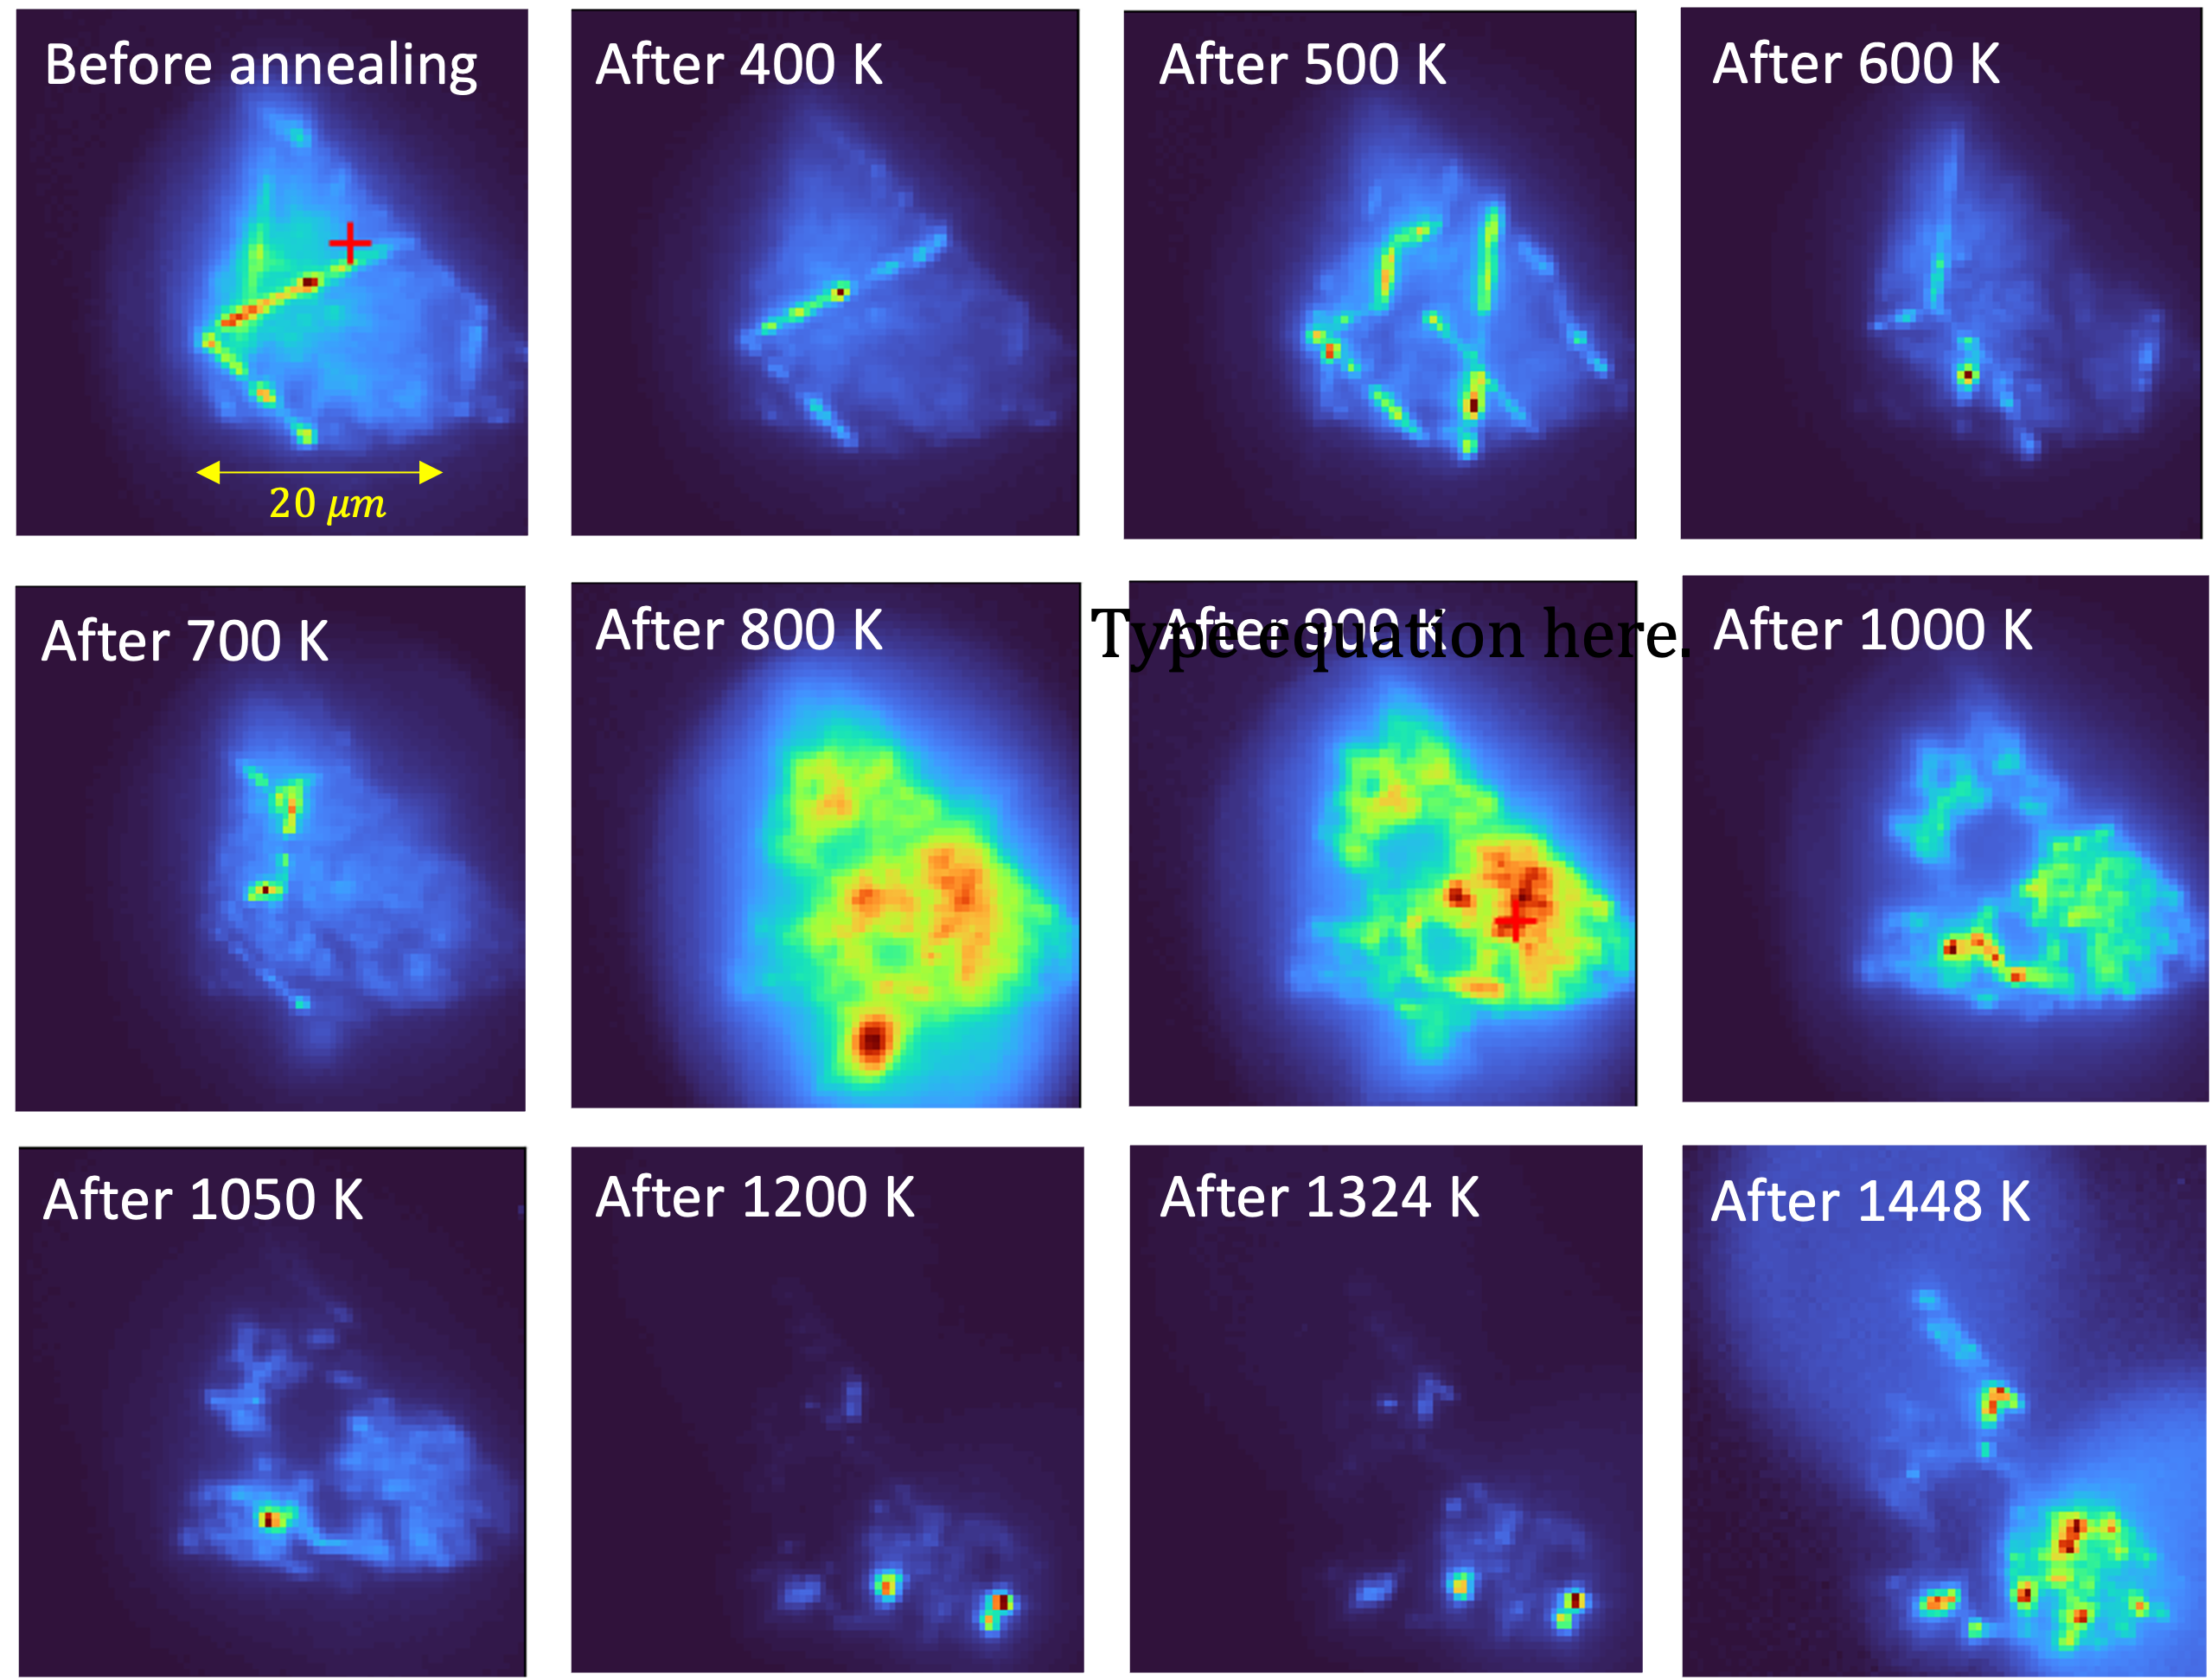
\includegraphics[width=\textwidth]{Figure/Chapter_five/hyperspectral_sequence.png}
%     \caption{Sequence of hyperspectral PL maps of an hBN-encapsulated WS$_2$ flake (chip 3-2) at $T \approx 4$~K, recorded after annealing at temperatures from 400~K to 1448~K (emission integrated over 600--650~nm). The progressive evolution shows initial spectral stability, emergence of bright defect spots at 800--900~K, maximum brightness near 900--1050~K, and gradual decrease at higher temperatures. The scale bar indicates 20~$\mu$m.}
%     \label{fig:hyperspectral_sequence}
% \end{figure}
% Source: CSI 2nd year report (methodology.tex), Fig. 17.
%   Chip 3-2, T~4K, emission integrated 600-650 nm.
%   Grid of 12 PL maps: Before annealing, 400K, 500K, 600K, 700K, 800K, 900K, 1000K, 1050K, 1200K, 1324K, 1448K.
%   False-color scale (blue=low, red=high), consistent spatial + color scale, temperature labeled on each panel.

By tracking the A-exciton peak energy at a fixed spatial position as a function of annealing temperature, we observe a progressive redshift of the exciton energy. Fig.~\ref{fig:exciton_energy_map} shows the extracted exciton peak energies at two representative pixels across the annealing sequence. A monotonic redshift of $\sim$75~meV is observed between the as-prepared sample and the sample after 1400~K annealing. This redshift is not spatially uniform: different positions on the flake exhibit different degrees of redshift, reflecting the spatial inhomogeneity of the thermally induced structural modifications (strain, partial decomposition, and potentially local composition changes).

% \begin{figure}[htbp]
%     \centering
%     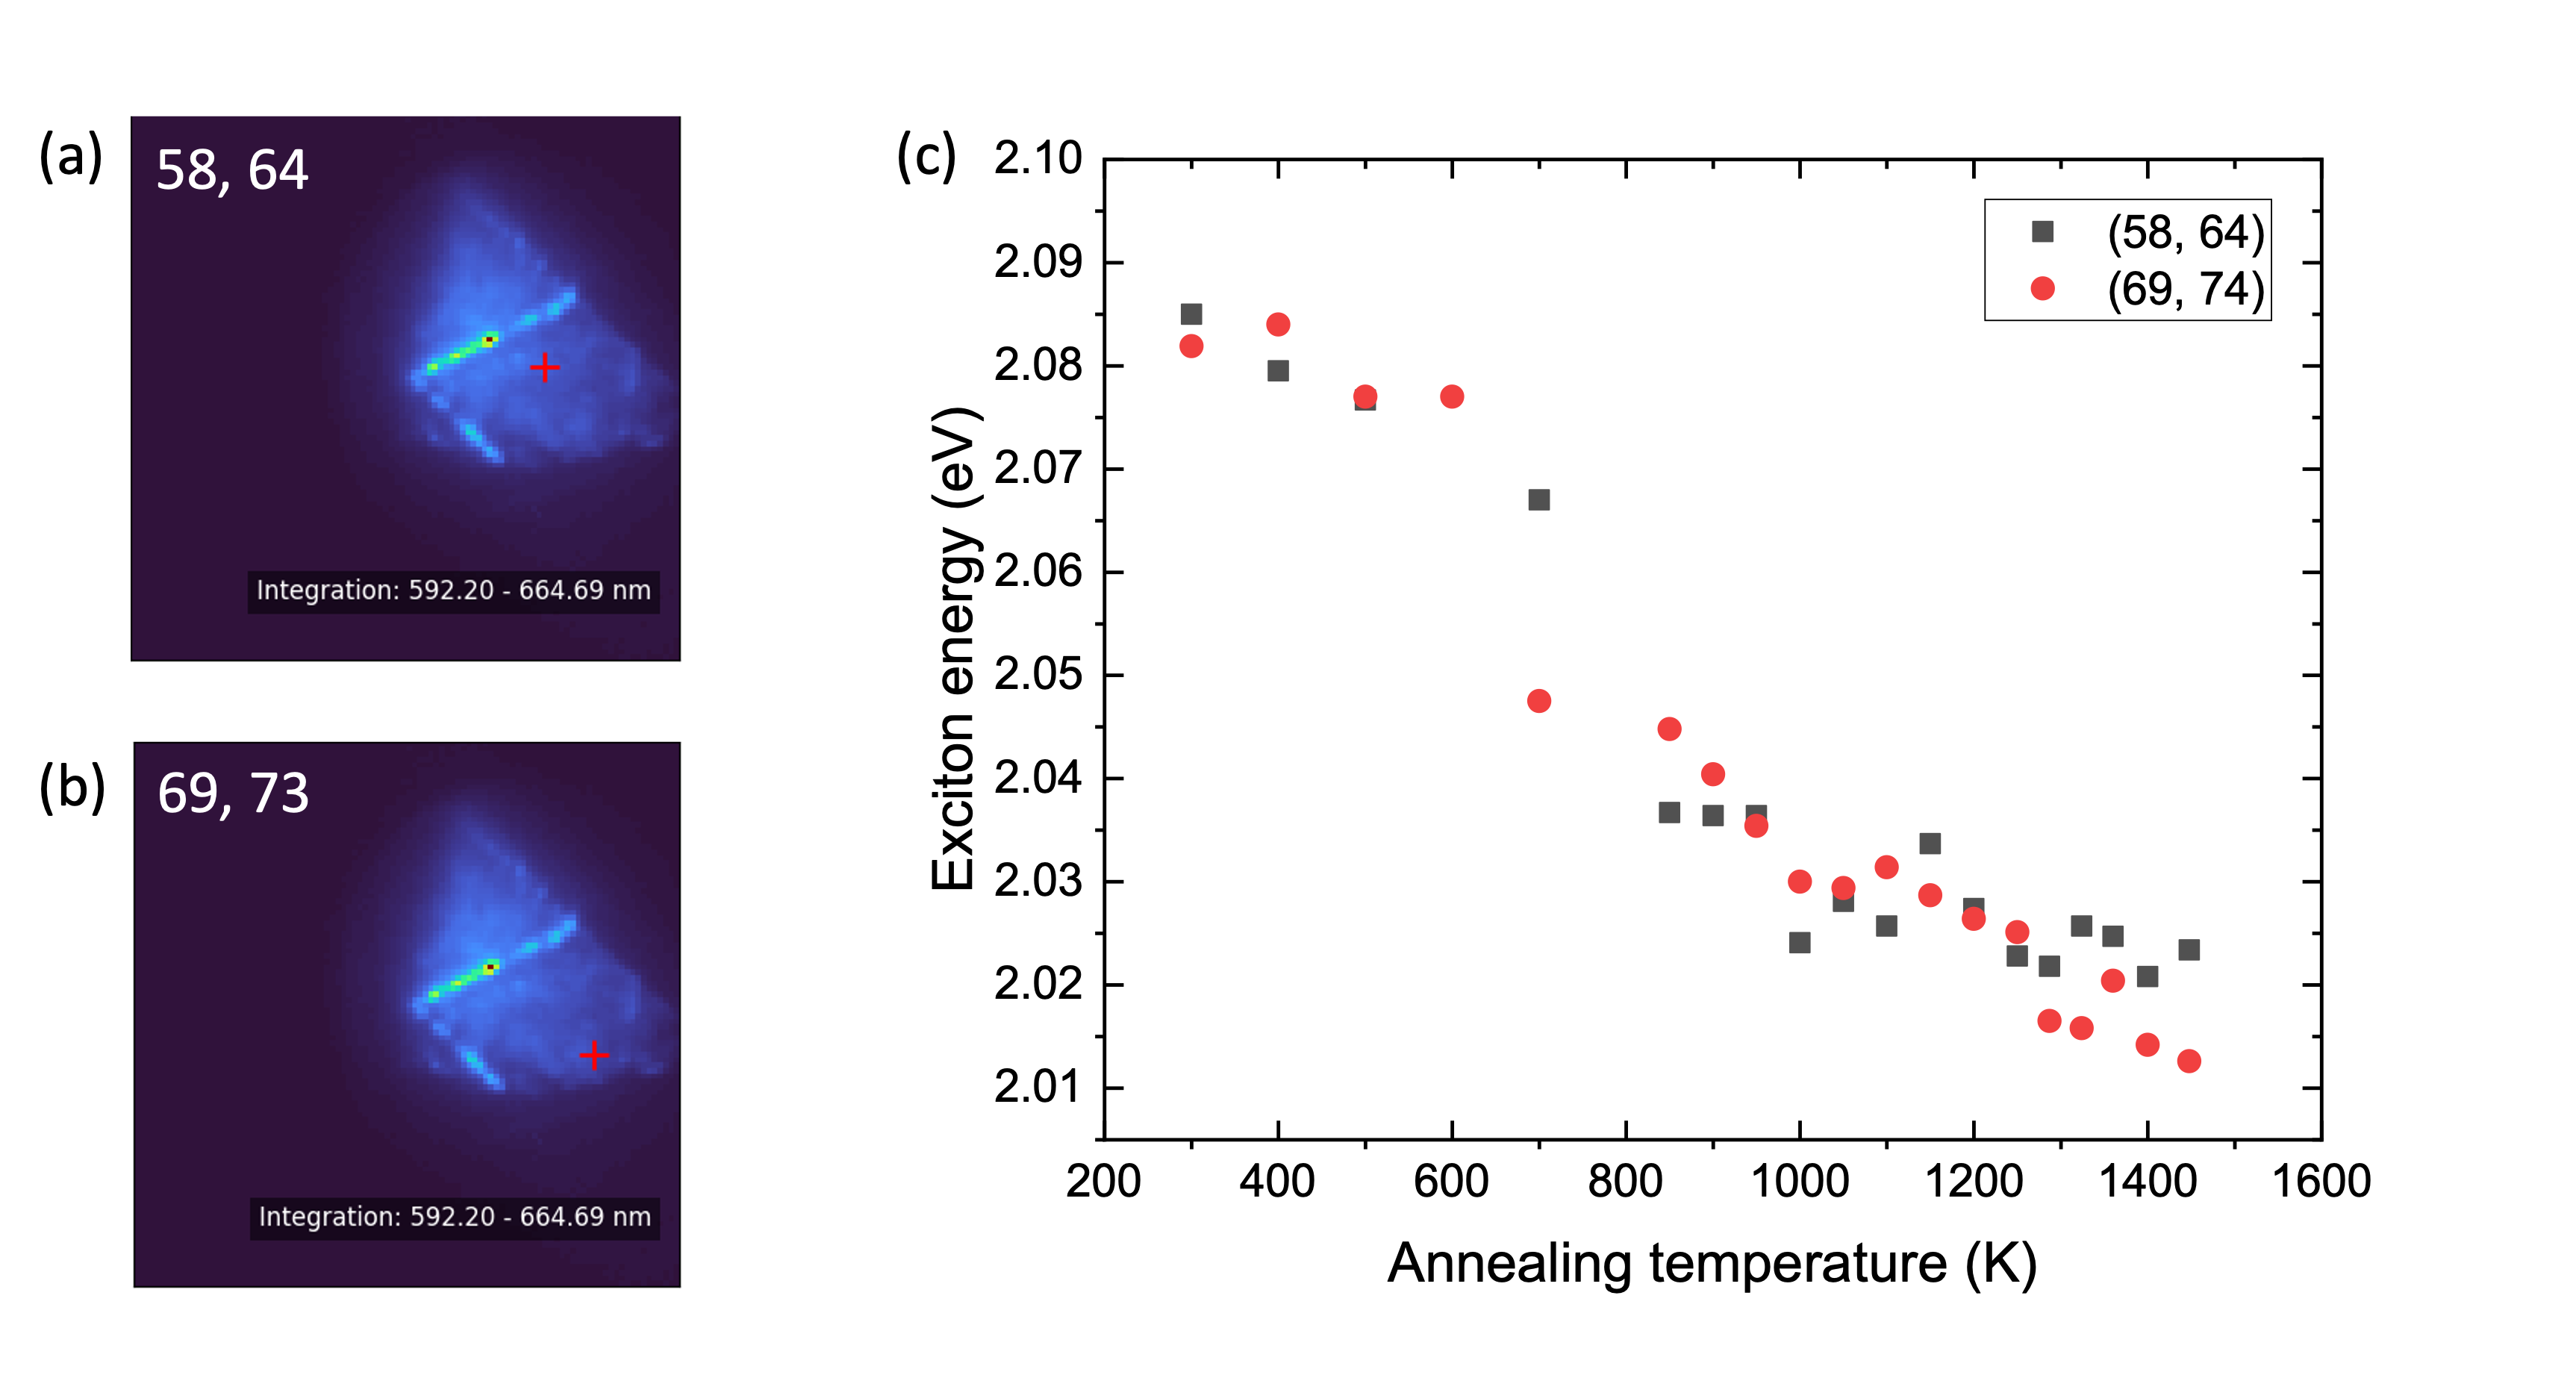
\includegraphics[width=0.7\textwidth]{Figure/Chapter_five/exciton_energy_map.png}
%     \caption{Evolution of the A-exciton energy as a function of annealing temperature, extracted at two representative spatial positions (pixels 58,64 and 69,74) from the hyperspectral PL datacube. A progressive redshift of $\sim$75~meV is observed after 1400~K annealing, reflecting the accumulation of local strain in the WS$_2$ lattice.}
%     \label{fig:exciton_energy_map}
% \end{figure}
% Source: CSI 2nd year report (methodology.tex), Fig. 18(c).
%   Scatter/line plot: exciton energy (eV, y-axis) vs. annealing temperature (K, x-axis, 200-1600K).
%   Two data series for pixels (58,64) and (69,74). Square and circle markers in different colors.

Confocal PL mapping on chip 4-2, shown in Fig.~\ref{fig:confocal_maps}, provides complementary spatial information with higher resolution. The maps recorded before annealing and after 500~K, 600~K, and 700~K annealing steps show the evolution of the total PL intensity distribution across the flake. The initial uniform emission is gradually replaced by a spatially structured pattern after annealing, with some regions brightening (indicating increased defect density) and others darkening. The exciton peak energy extracted from the pixel-by-pixel spectra confirms a progressive redshift with annealing temperature, consistent with the wide-field measurements.

% \begin{figure}[htbp]
%     \centering
%     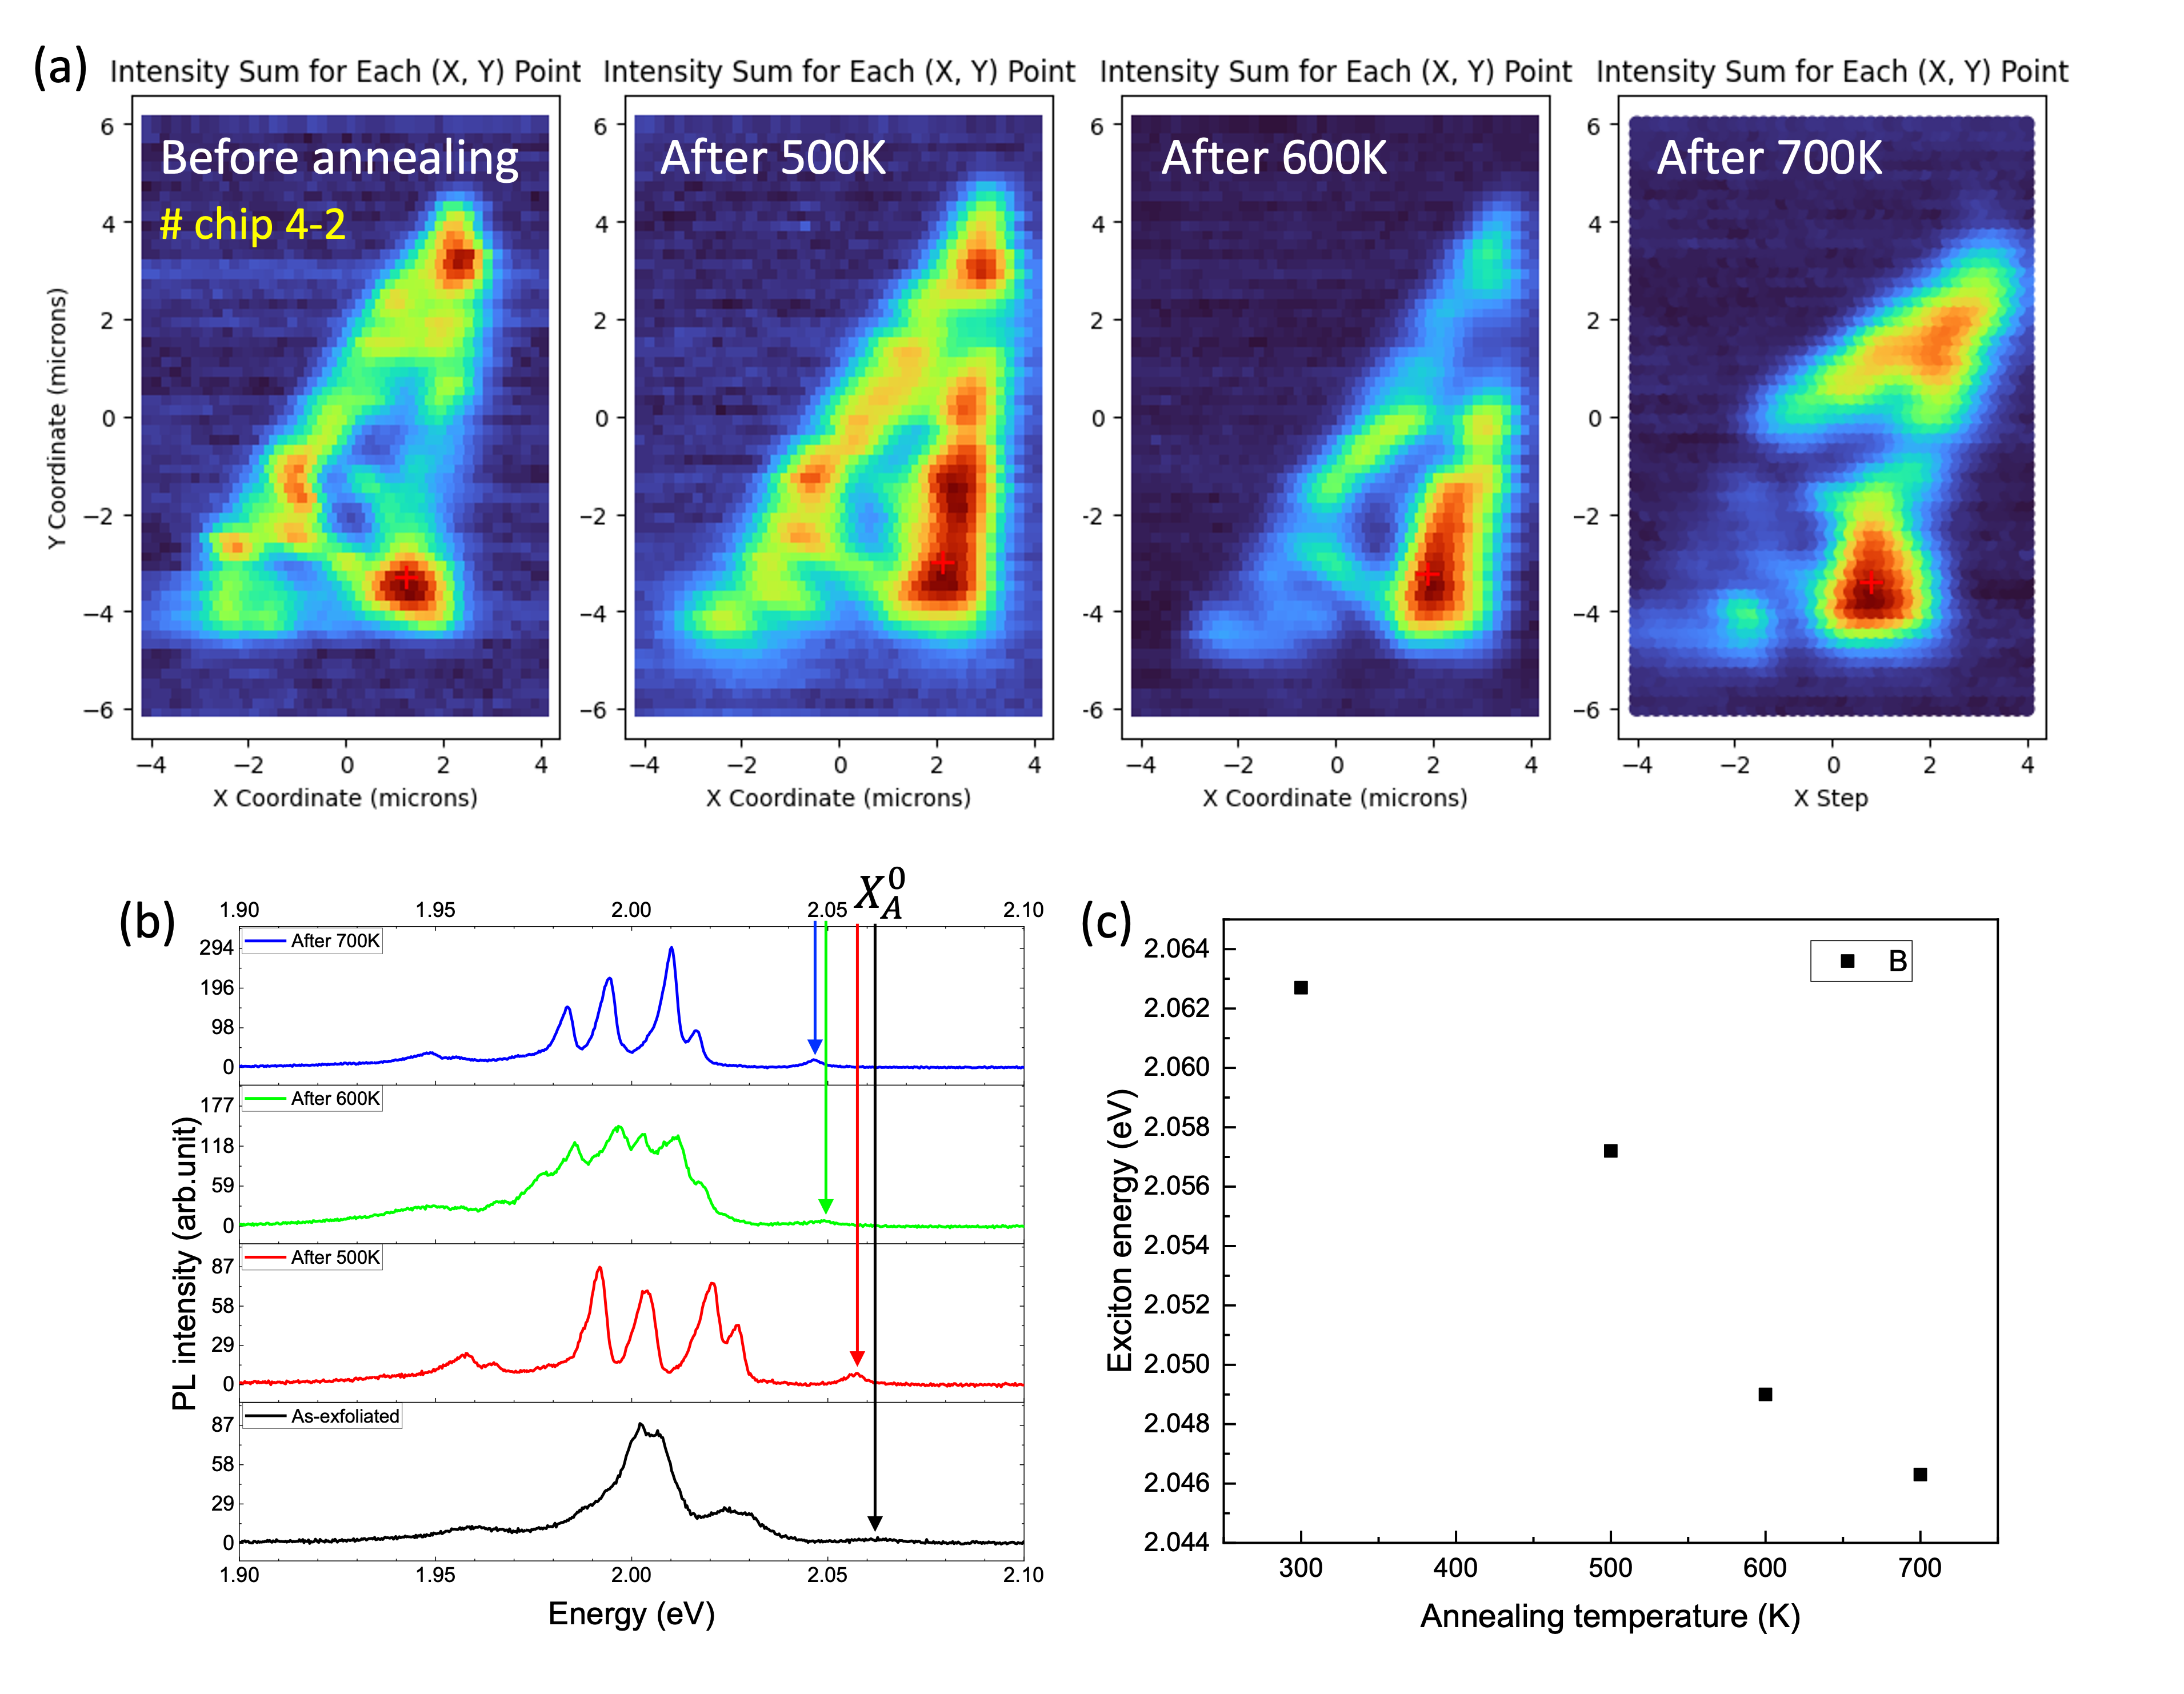
\includegraphics[width=\textwidth]{Figure/Chapter_five/confocal_maps.png}
%     \caption{Confocal PL maps of chip 4-2 before annealing and after 500~K, 600~K, and 700~K annealing steps, showing the evolution of the total PL intensity distribution. The exciton peak energy extracted from pixel-by-pixel spectra (not shown) confirms a progressive redshift consistent with the wide-field hyperspectral results.}
%     \label{fig:confocal_maps}
% \end{figure}
% Source: CSI 2nd year report (methodology.tex), Fig. 20(a).
%   Chip 4-2. 4-panel figure: before annealing, 500K, 600K, 700K.
%   Confocal PL intensity maps. Same spatial scale and color scale across all panels.


\subsection{Localization of Low-Energy Emission after High-Temperature Annealing}
\label{subsec:Localization of Low-Energy Emission after High-Temperature Annealing}

The hyperspectral dataset recorded on chip~3-2 was re-analyzed with the spectral integration window shifted to approximately 1.85~eV, below the $X_L$ emission range. Above 1150~K annealing, a low-energy peak emerges at two spatially distinct positions within the flake. Fig.~\ref{fig:hyper_low_peak} summarizes the spectral evolution at both positions.

At pixel~(77, 72), the low-energy peak appears after the 1150~K annealing step and redshifts progressively with increasing temperature. Its intensity increases and reaches a maximum after the 1250~K anneal, then decreases at higher temperatures and eventually disappears upon further annealing. A qualitatively identical behavior is observed at pixel~(61, 69): the emission appears above 1150~K, peaks at 1250~K, and vanishes at higher temperatures. The energies of the two peaks after the 1250~K anneal are approximately 1.854~eV and 1.827~eV, respectively.

The spatial localization of this emission to two fixed positions---which remain unchanged across successive annealing steps---and its appearance only above a well-defined annealing threshold indicate that these spots correspond to specific structural sites within the WS$_2$ flake.

% \begin{figure}[htbp]
%     \centering
%     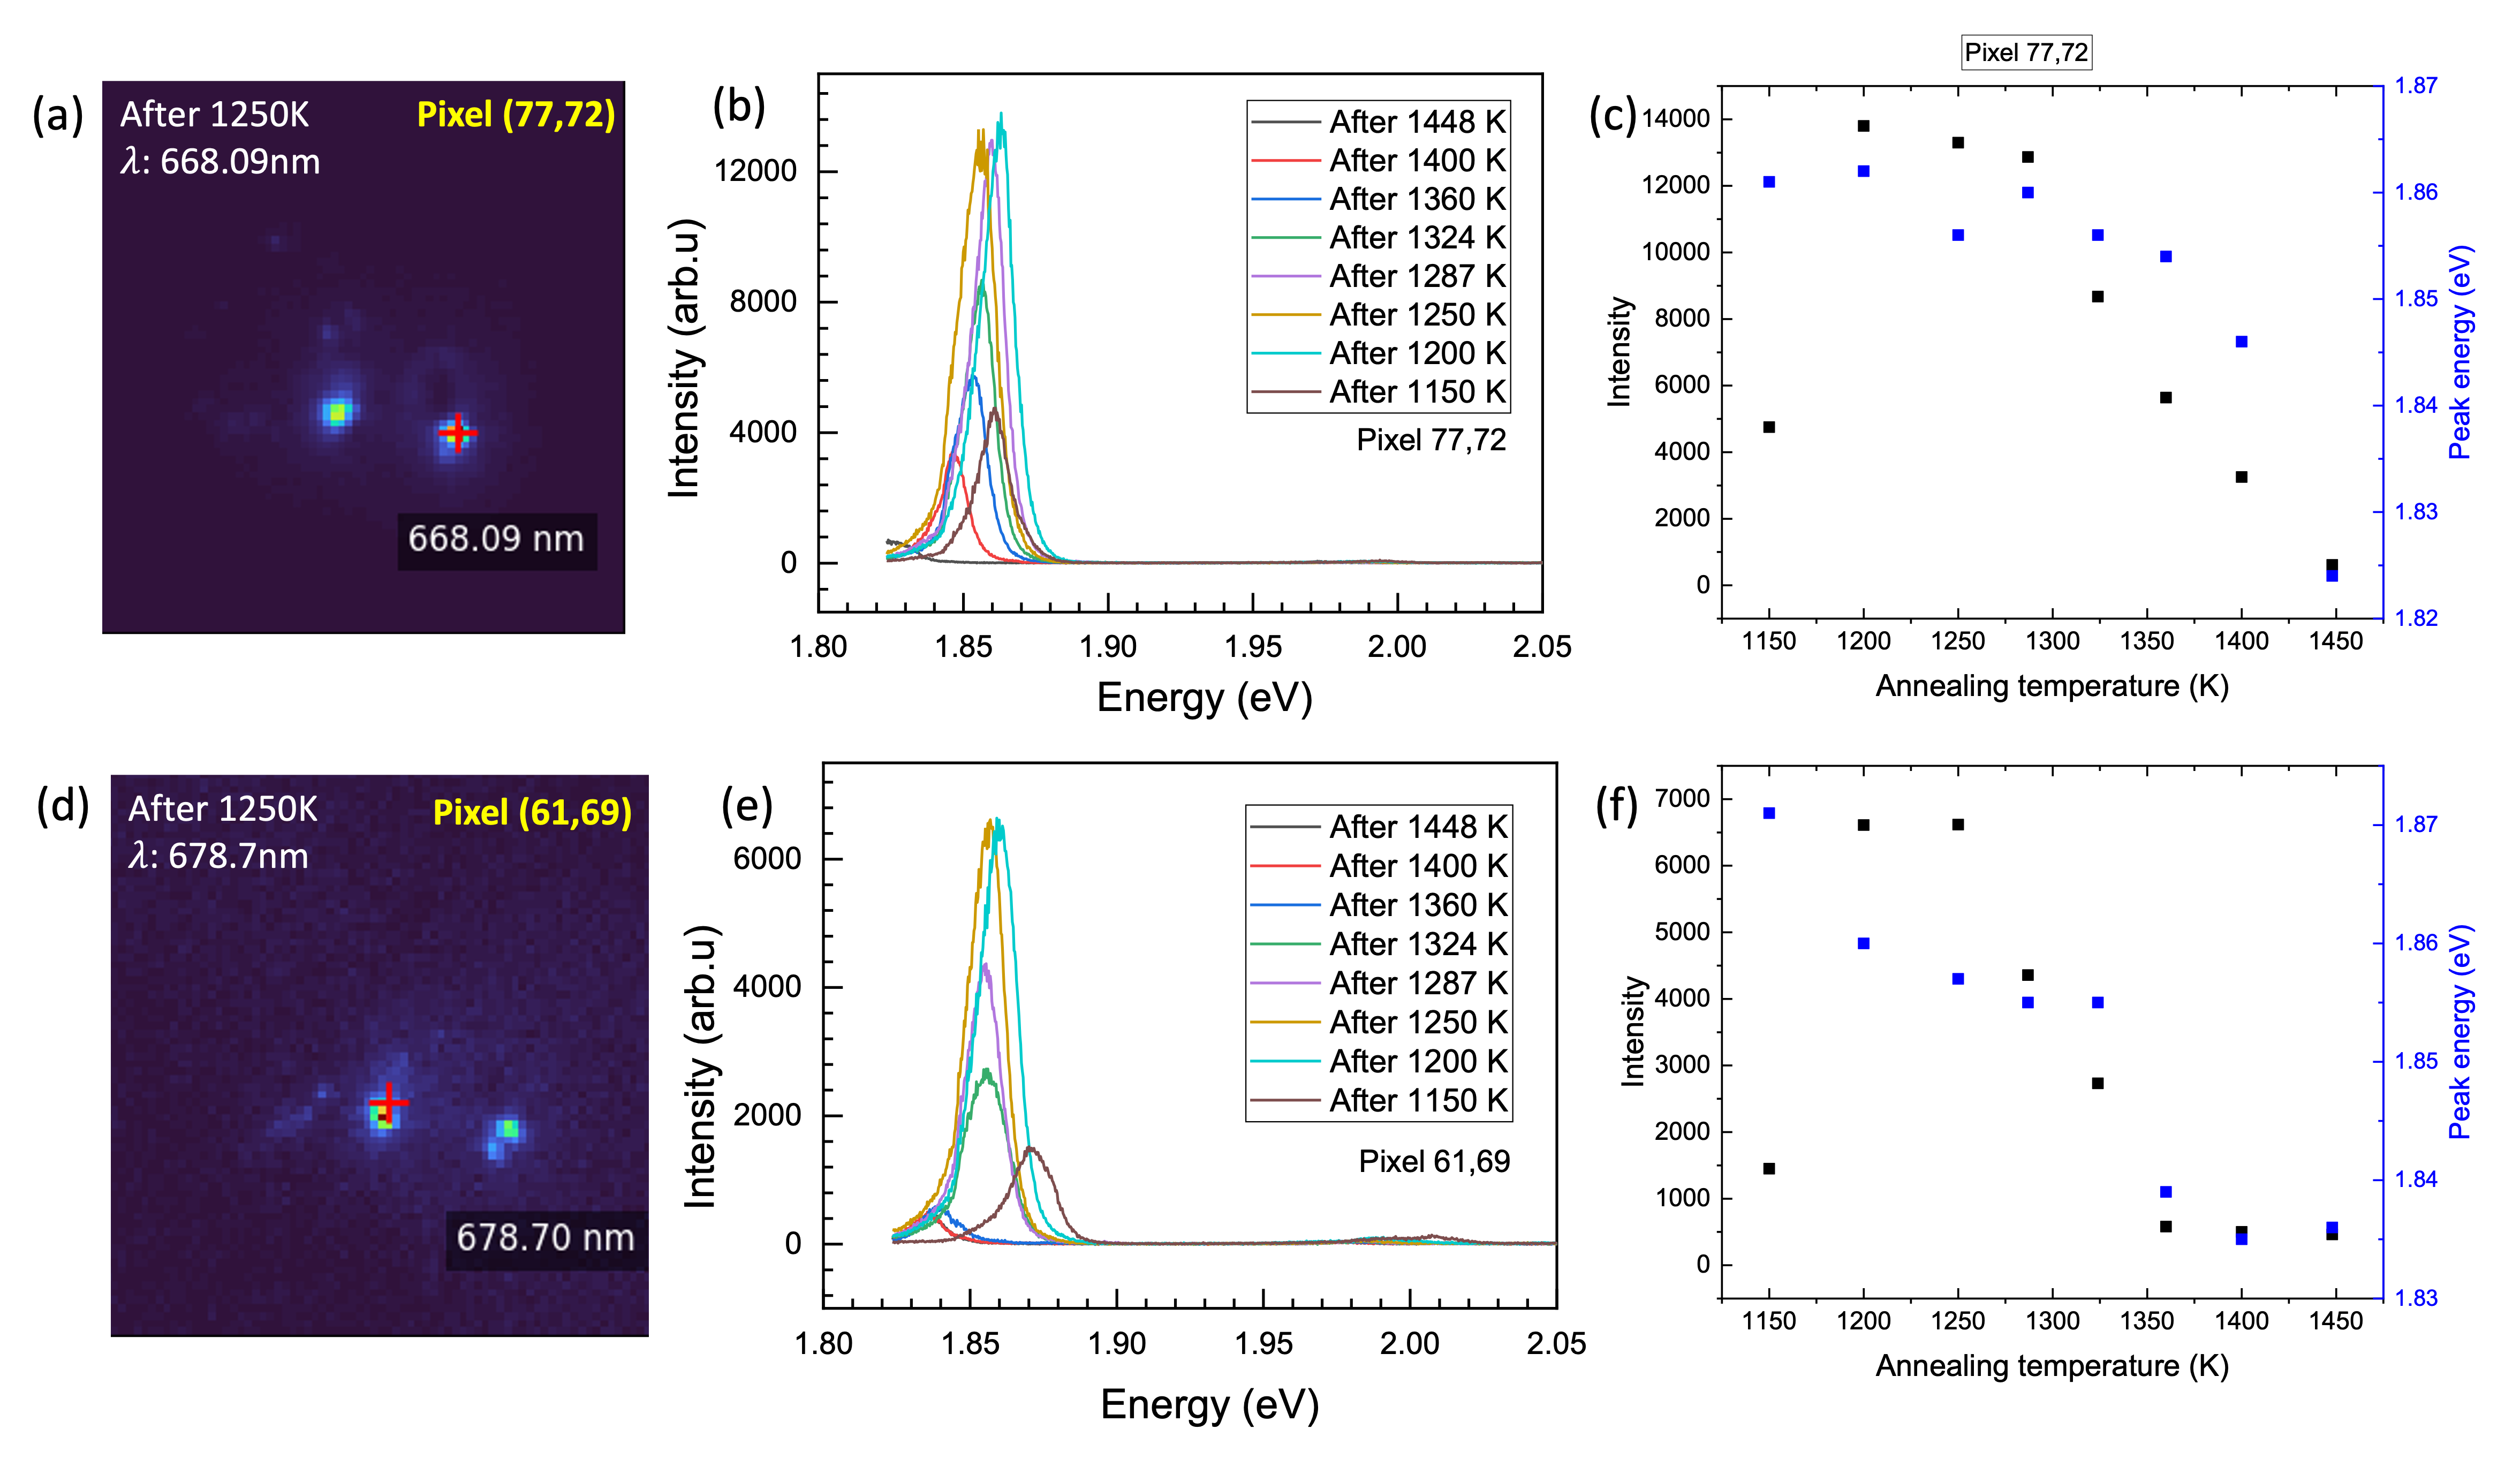
\includegraphics[width=\textwidth]{Figure/Chapter_five/hyper_low_peak.png}
%     \caption{Emergence and evolution of low-energy emission at two localized positions in chip~3-2 above 1150~K annealing. (a--c) Results for pixel~(77, 72): (a) hyperspectral PL map after 1250~K annealing with the selected pixel marked, (b) PL spectra showing the evolution of the low-energy peak between 1150~K and 1448~K, and (c) peak intensity (left axis) and energy (right axis) as a function of annealing temperature. (d--f) Corresponding results for pixel~(61, 69): (d) hyperspectral PL map after 1250~K annealing, (e) PL spectral evolution, and (f) peak intensity and energy as a function of annealing temperature.}
%     \label{fig:hyper_low_peak}
% \end{figure}
% Source: CSI 2nd year report (methodology.tex), figure 'hyper_low_peak'.
%   Chip 3-2, spectral integration window ~1.85 eV (below X_L range).
%   Pixel (77,72): peak ~1.854 eV at 1250K max. Pixel (61,69): peak ~1.827 eV at 1250K max.
%   6-panel layout: (a-c) pixel (77,72), (d-f) pixel (61,69).
%   Each set: hyperspectral map with pixel marked | PL spectra evolution 1150-1448K | intensity+energy vs T.


\subsection{Strain Quantification from PL and Raman Gauge Factors}
\label{subsec:Strain Quantification from PL and Raman Gauge Factors}

To investigate the origin of the spatial inhomogeneities revealed by the hyperspectral measurements, we performed correlated room-temperature PL and Raman measurements on chip~3-5 before and after annealing to 1500~K. Fig.~\ref{fig:plmap_RT_chip3-5} shows PL maps recorded at room temperature. Before annealing, the PL emission is spatially homogeneous in terms of peak energy distribution. After annealing at 1500~K, the PL maps reveal significant spatial inhomogeneity: both the PL intensity and the exciton peak energy vary across the flake, indicating that high-temperature annealing introduced local structural modifications.

To characterize these modifications quantitatively, three representative spots were selected from the post-annealing PL map (Fig.~\ref{fig:chip35_spots}(a)): Spot~1, which shows no spectral shift and serves as the reference, and Spots~2 and 3, which exhibit progressively larger redshifts. PL spectra recorded at room temperature (Fig.~\ref{fig:chip35_spots}(b)) show a clear redshift of the A-exciton peak at Spots~2 and 3. Raman spectra at the same positions (Fig.~\ref{fig:chip35_spots}(c)) reveal the two characteristic vibrational modes of WS$_2$: the in-plane $E_{2g}$ mode and the out-of-plane $A_{1g}$ mode. Both modes shift to lower wavenumber after annealing, with the $E_{2g}$ mode exhibiting a larger absolute shift, consistent with its higher sensitivity to in-plane strain~\cite{wang-2020}.

The local strain at each spot is estimated from the measured spectral shifts using the gauge factors reported in the literature~\cite{wang-2020,wang-2016}:
\begin{equation}
\varepsilon_{\mathrm{Raman}} = \frac{\Delta\omega_{E_{2g}}}{d\omega_{E_{2g}}/d\varepsilon}, \qquad \varepsilon_{\mathrm{PL}} = \frac{\Delta E_X}{dE_X/d\varepsilon},
\label{eq:strain_gauge}
\end{equation}
where $d\omega_{E_{2g}}/d\varepsilon \approx -2.05~\mathrm{cm^{-1}/\%}$ and $dE_X/d\varepsilon \approx -58.7~\mathrm{meV/\%}$ are the Raman and PL gauge factors for WS$_2$, respectively. The resulting strain estimates are summarized in Table~\ref{tab:pl_raman_strain}.

\begin{table}[htbp]
\centering
\caption{Room-temperature PL and Raman $E_{2g}$ results at three representative spots of chip~3-5 after 1500~K annealing. Strain estimates use the PL A-exciton gauge factor $dE_X/d\varepsilon = -58.7~\mathrm{meV/\%}$ and the Raman gauge factor $d\omega_{E_{2g}}/d\varepsilon = -2.05~\mathrm{cm^{-1}/\%}$~\cite{wang-2020,wang-2016}.}
\label{tab:pl_raman_strain}
\begin{tabular}{c c c c c c c}
\hline
Spot & \multicolumn{3}{c}{PL (A exciton)} & \multicolumn{3}{c}{Raman $E_{2g}$} \\
\cline{2-7}
 & Peak (eV) & $\Delta E$ (meV) & $\varepsilon_{\mathrm{PL}}$ (\%)
 & Peak (cm$^{-1}$) & $\Delta\omega$ (cm$^{-1}$) & $\varepsilon_{E_{2g}}$ (\%) \\
\hline
1 & 1.99655 & \phantom{$-$}0.00 & 0.00 & 357.750 & \phantom{$-$}0.000 & 0.00 \\
2 & 1.93396 & $-$62.59 & 1.07 & 355.649 & $-$2.100 & 1.02 \\
3 & 1.90055 & $-$96.00 & 1.64 & 354.864 & $-$2.886 & 1.41 \\
\hline
\end{tabular}
\end{table}

The strain estimates from PL and Raman are broadly consistent at each spot: Spot~2 yields $\varepsilon_{\mathrm{PL}} \approx 1.07\%$ and $\varepsilon_{E_{2g}} \approx 1.02\%$, while Spot~3 yields $\varepsilon_{\mathrm{PL}} \approx 1.64\%$ and $\varepsilon_{E_{2g}} \approx 1.41\%$. The small discrepancies between the two estimates can be attributed to local doping, defect states, anisotropic stress distributions, or the different sensitivities of the PL and Raman probes to local structural modifications~\cite{wang-2020}. The correlated redshifts of the exciton peak and the $E_{2g}$ phonon mode at Spots~2 and 3 indicate that high-temperature annealing introduces tensile strain of order 1--2\% at localized positions within the flake, simultaneously reducing the optical bandgap and softening the in-plane vibrational modes.

% \begin{figure}[htbp]
%     \centering
%     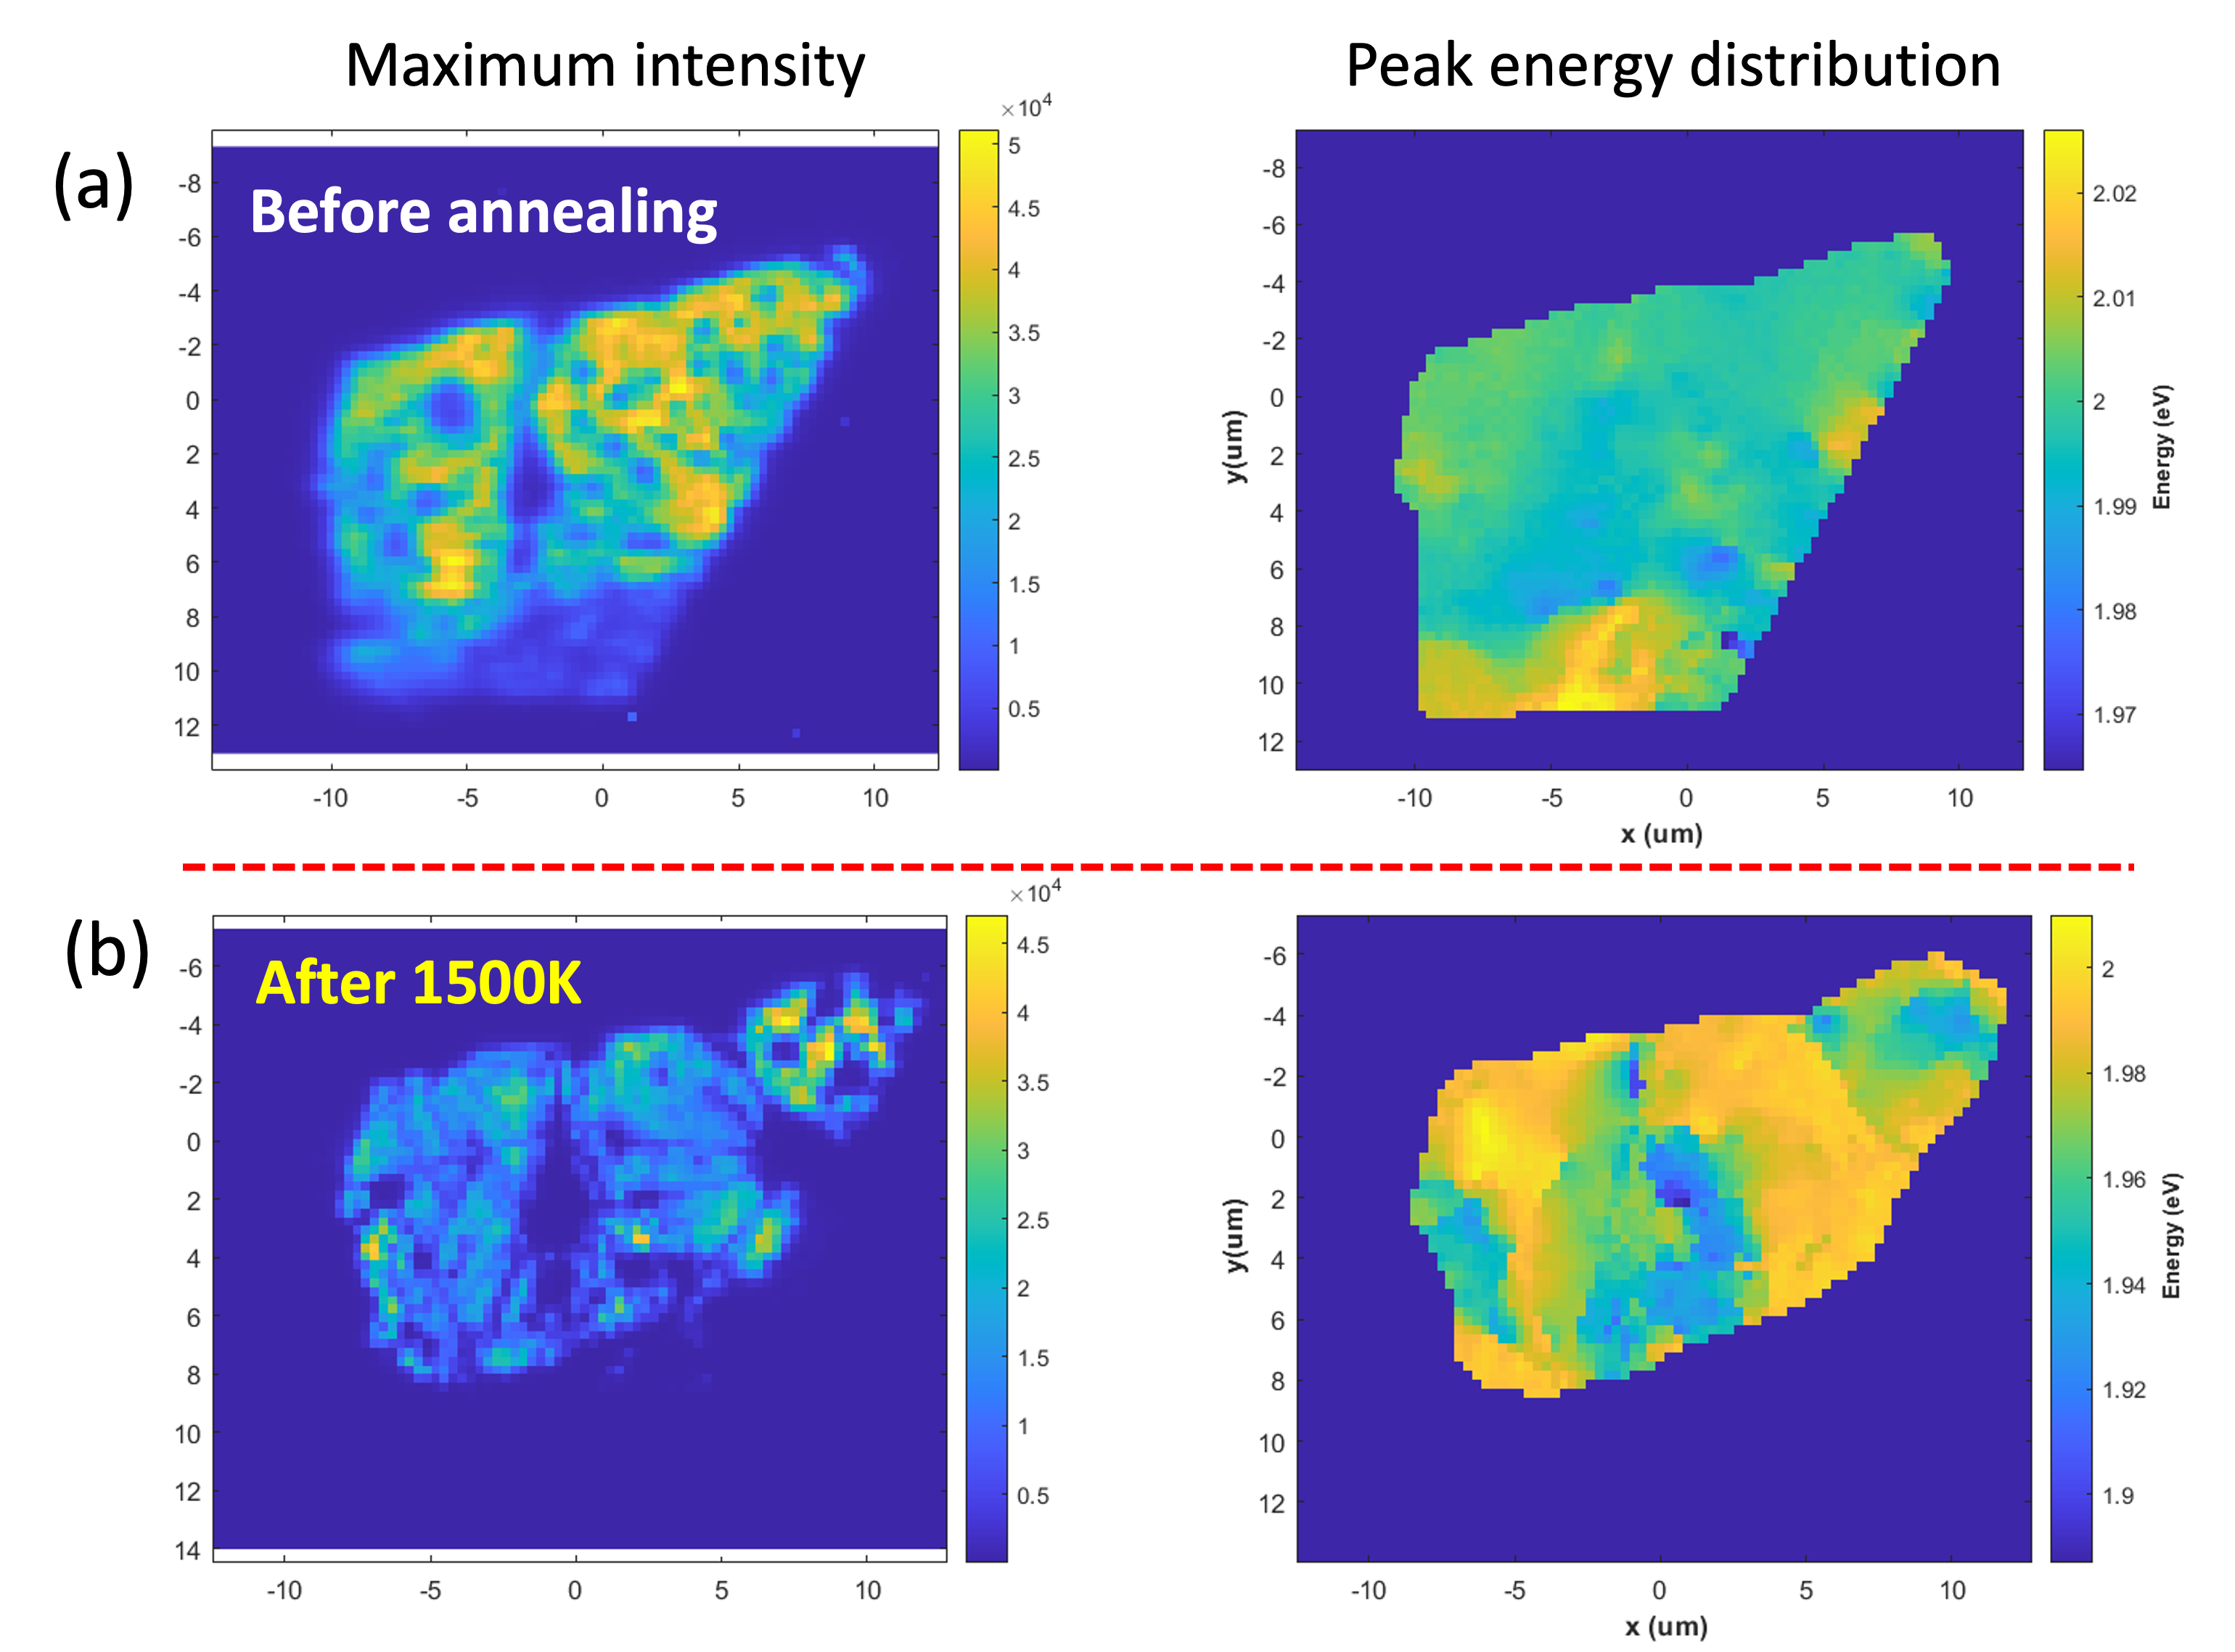
\includegraphics[width=\textwidth]{Figure/Chapter_five/plmap_RT_chip3-5.png}
%     \caption{Room-temperature PL maps of chip~3-5 (a) before annealing, showing a spatially homogeneous peak energy distribution, and (b) after annealing at 1500~K, revealing significant spatial inhomogeneity in both PL intensity and exciton peak energy.}
%     \label{fig:plmap_RT_chip3-5}
% \end{figure}
% Source: CSI 2nd year report (methodology.tex), figure 'plmap_RT_chip3-5'.
%   Chip 3-5, room temperature. 2-panel: (a) before annealing (uniform), (b) after 1500K (inhomogeneous).
%   Show both PL intensity and peak energy maps if possible.

% \begin{figure}[htbp]
%     \centering
%     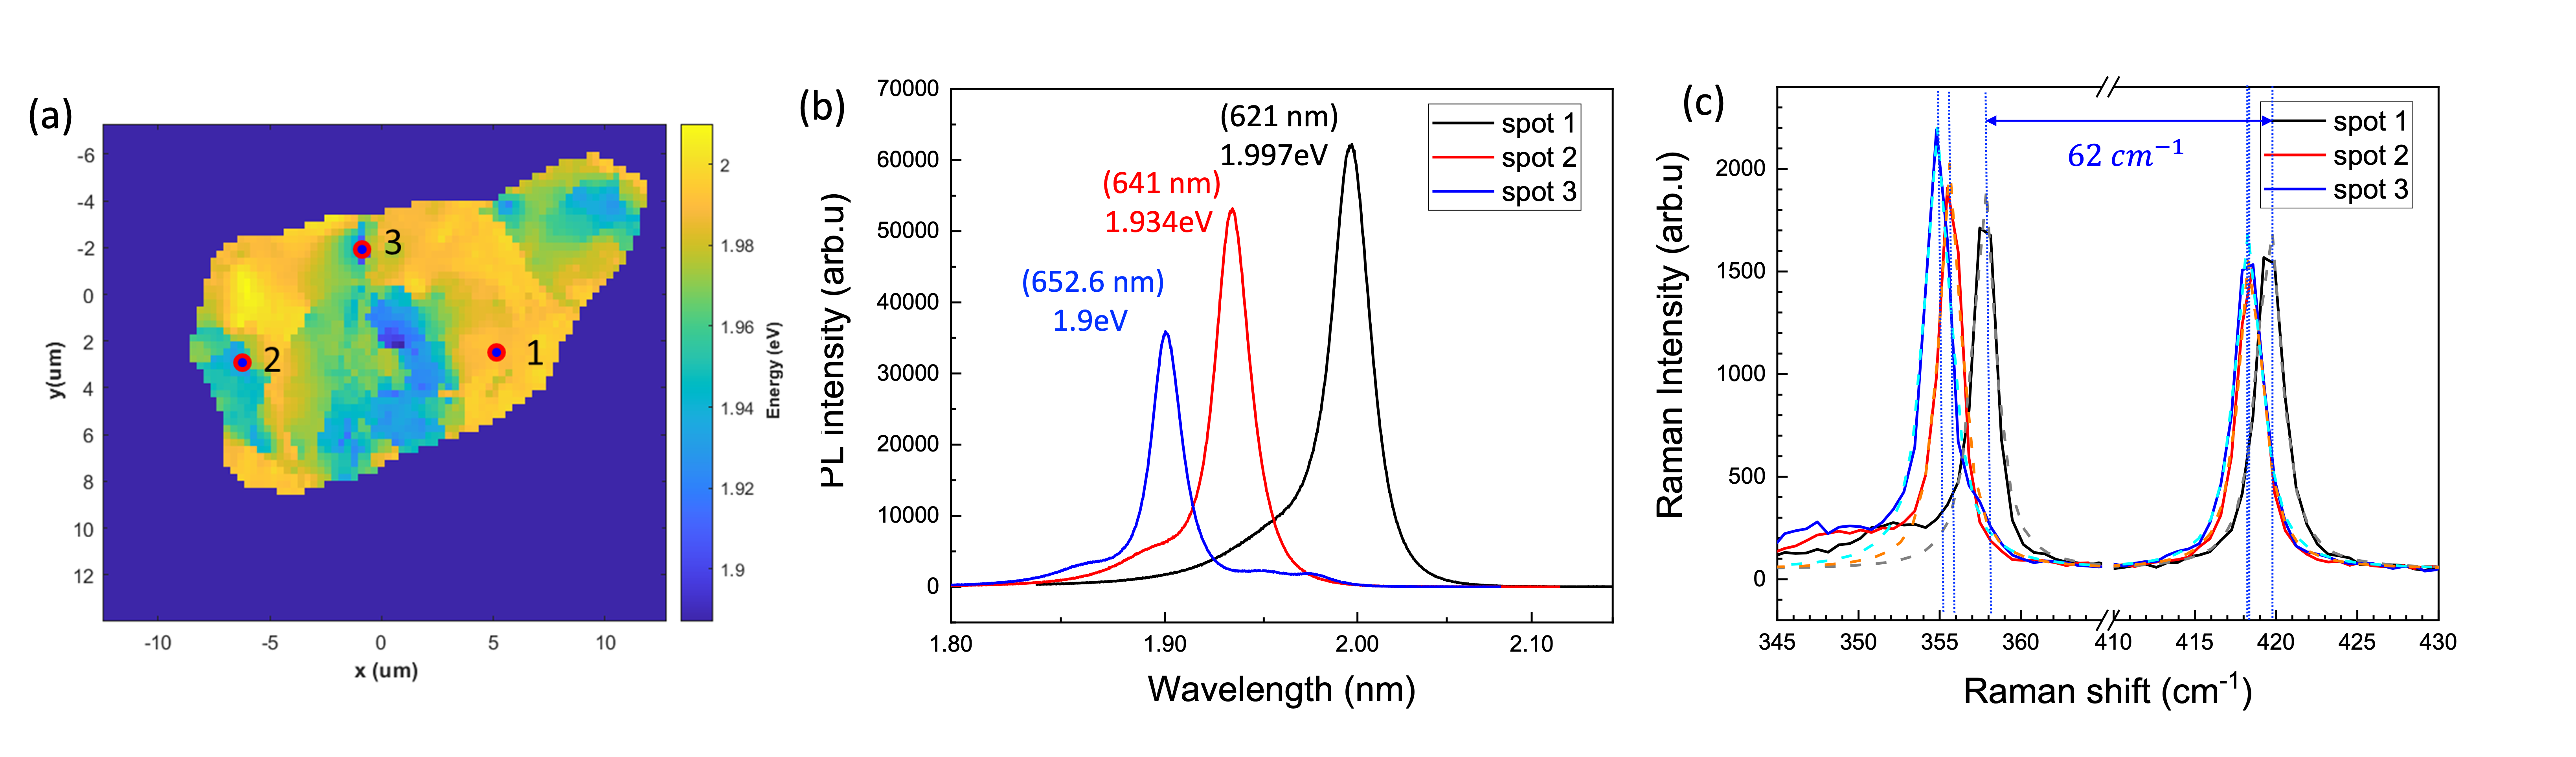
\includegraphics[width=\textwidth]{Figure/Chapter_five/chip35_spots.png}
%     \caption{(a) PL map of chip~3-5 after 1500~K annealing with three representative spots indicated. (b) Room-temperature PL spectra at the three spots, showing progressive redshift of the A-exciton peak at Spots~2 and 3 relative to the reference Spot~1. (c) Raman spectra at the same spots under 473~nm laser excitation, showing redshifts of the $E_{2g}$ and $A_{1g}$ modes.}
%     \label{fig:chip35_spots}
% \end{figure}
% Source: CSI 2nd year report (methodology.tex), figure 'chip35_spots'.
%   Chip 3-5. 3-panel figure:
%   (a) PL map after 1500K annealing with Spots 1, 2, 3 marked.
%   (b) RT PL spectra at 3 spots. Spot 1: 1.99655 eV. Spot 2: 1.93396 eV. Spot 3: 1.90055 eV.
%   (c) Raman spectra at 3 spots (473 nm laser). Spot 1: E2g 357.750 cm^-1.
%       Spot 2: E2g 355.649 cm^-1. Spot 3: E2g 354.864 cm^-1.


\section{Conclusion}
\label{sec:ch5:Conclusion}

This chapter has presented a comprehensive characterization of the $X_D$ emission in hBN-encapsulated WS$_2$ monolayers, establishing its properties as a single-photon emitter and revealing the spatial and structural context of its formation.

$X_D$ emerges above $\sim$1100~K annealing temperature as a set of ultra-narrow emission peaks positioned 75--86~meV below the neutral exciton, with linewidths at or below the spectrometer resolution limit of $\approx 0.2$~meV at low excitation powers. The power-dependent linewidth narrowing and intensity saturation (with $P_\gamma = 2.73$~$\mu$W under pulsed 78~MHz excitation) confirm the two-level quantum emitter character of $X_D$.

PLE spectroscopy demonstrates unambiguously that $X_D$ is fed through the intrinsic optical resonances of WS$_2$ (A and B excitons and their excited states), ruling out contributions from hBN or SiC. The Stokes shift between the A-exciton absorption and the $X_D$ emission corresponds to a localization energy of $\sim$80--90~meV, slightly shallower than the $\sim$120~meV of $X_L$.

Time-resolved PL reveals a delayed onset of $\sim$200~ps (reflecting exciton diffusion and capture) followed by a single-exponential decay with $\tau \approx 0.9$~ns---approximately twice the lifetime of $X_L$ and nearly an order of magnitude longer than the bright excitonic complexes, consistent with a reduced oscillator strength of the defect-localized state. The long lifetime contributes to an estimated quantum yield of $\sim$5.25\%, among the highest reported for thermally activated 2D defect emitters.

Photon correlation measurements under pulsed excitation at 78~MHz yield $g^{(2)}(0) \approx 0.3$--0.4, well below the 0.5 threshold, providing unambiguous evidence of single-photon emission from $X_D$. The residual $g^{(2)}(0) > 0$ is attributed to background emission and a small number ($\lesssim 2$) of simultaneously active emitters within the diffraction-limited spot.

Hyperspectral PL imaging reveals the spatial evolution of the annealing-induced modifications across the WS$_2$ flake. Wide-field imaging of chip 3-2 shows a sequence from uniform emission before annealing to the emergence of localized bright spots in the 800--1000~K range, followed by a reduction in emission at higher temperatures. A progressive redshift of the exciton energy of up to $\sim$75~meV is observed across the annealing sequence (up to $\sim$1400~K), reflecting the spatial inhomogeneity of the thermally induced structural modifications. Confocal PL mapping on chip 4-2 confirms the spatially structured evolution of the emission with annealing temperature at higher spatial resolution. Above 1150~K, low-energy emission localizes at two fixed positions within the flake, with peak energies after the 1250~K anneal of approximately 1.854~eV and 1.827~eV. Correlated PL and Raman measurements on chip~3-5 after 1500~K annealing reveal local tensile strain of 1--2\% at selected positions, consistent with the spatially inhomogeneous bandgap reductions observed in the PL maps.

Taken together, the results of this chapter establish that controlled in-situ thermal annealing of hBN-encapsulated WS$_2$ monolayers is a robust approach to creating single-photon emitters with excellent spectral purity and long radiative lifetime. The approach requires no lithographic processing, ion beams, or chemical functionalization---only thermal energy---making it compatible with clean-room-free sample environments and with the sensitive cryogenic measurements needed to characterize quantum optical properties. The central remaining challenges are the spatial control of emitter placement, the extension of operating temperature, and the demonstration of photon indistinguishability, which will require further reduction of spectral diffusion and integration of $X_D$ emitters into photonic cavities.



% ---- bibliography

\printbibliography[heading=subbibintoc]
% \bibliographystyle{apalike}
% \bibliography{bib_thesis}



\end{document}
